% REMEMBER: You must not plagiarise anything in your report. Be extremely careful.

\documentclass{l4proj}

    
%
% put any additional packages here
%

\usepackage{pifont}
\newcommand{\cmark}{\ding{51}}
\newcommand{\xmark}{\ding{55}}

\begin{document}

%==============================================================================
%% METADATA
\title{Heart Rate Recovery Tracking for Fitness on a Smartwatch}
\author{Nathan Hutchison}
\date{February 2, 2024}

\maketitle

%==============================================================================
%% ABSTRACT
\begin{abstract}
    Every abstract follows a similar pattern. Motivate; set aims; describe work; explain results.
    \vskip 0.5em
    ``XYZ is bad. This project investigated ABC to determine if it was better. 
    ABC used XXX and YYY to implement ZZZ. This is particularly interesting as XXX and YYY have
    never been used together. It was found that  
    ABC was 20\% better than XYZ, though it caused rabies in half of subjects.''
\end{abstract}

%==============================================================================

% EDUCATION REUSE CONSENT FORM
% If you consent to your project being shown to future students for educational purposes
% then insert your name and the date below to  sign the education use form that appears in the front of the document. 
% You must explicitly give consent if you wish to do so.
% If you sign, your project may be included in the Hall of Fame if it scores particularly highly.
%
% Please note that you are under no obligation to sign 
% this declaration, but doing so would help future students.
%
\def\consentname {Nathan Hutchison} % your full name
\def\consentdate {05 February 2024} % the date you agree
%
\educationalconsent


%==============================================================================
\tableofcontents

%==============================================================================
%% Notes on formatting
%==============================================================================
% The first page, abstract and table of contents are numbered using Roman numerals and are not
% included in the page count. 
%
% From now on pages are numbered
% using Arabic numerals. Therefore, immediately after the first call to \chapter we need the call
% \pagenumbering{arabic} and this should be called once only in the document. 
%
% Do not alter the bibliography style.
%
% The first Chapter should then be on page 1. You are allowed 40 pages for a 40 credit project and 30 pages for a 
% 20 credit report. This includes everything numbered in Arabic numerals (excluding front matter) up
% to but excluding the appendices and bibliography.
%
% You must not alter text size (it is currently 10pt) or alter margins or spacing.
%
%
%==================================================================================================================================
%
% IMPORTANT
% The chapter headings here are **suggestions**. You don't have to follow this model if
% it doesn't fit your project. Every project should have an introduction and conclusion,
% however. 
%
%==================================================================================================================================
\chapter{Introduction}
\label{sec:introduction}

% reset page numbering. Don't remove this!
\pagenumbering{arabic} 

\section{Motivation}
\label{sec:motivation}

In an era built on rapid technological advancements, there has been a recent explosion of innovative technology proving revolutionary in the monitoring and managing of an individual’s health. Fitness tracking technology has become an increasingly vast market, with a huge increase in people using fitness statistics to ensure they remain active and healthy in their day-to-day lives. However, while physical fitness can be easily measured through distance run or weight lifted, one aspect of fitness often overlooked is your heart health. 

Heart Rate Recovery (HRR) strongly indicates overall cardiovascular health and fitness. However many current fitness tracking applications strongly focus on tracking the physical activity itself through metrics such as distance run and lack HRR readings built in or make it so complex to view these readings that many users will be left unaware they even exist. 

By developing a smartwatch application that prioritises Heart Rate Recovery, I aim to bridge this gap in fitness tracking and bring heart health to the forefront of a user’s fitness tracking experience. This empowers individuals to have a clear and visual representation of their cardiovascular health, with the potential to lead to more effective workouts and a healthier lifestyle.

Furthermore, the convenience of having this application built into a smartwatch means users can view their Heart Rate Recovery at any time without having to use complex equipment or carry their phone about while exercising.

\section{Aim}
\label{sec:aim}

This project aims to develop a smartwatch application that allows users to intuitively track their Heart Rate Recovery during a workout, providing them with useful insight into their overall heart health. Results will be represented in visual graphs with a strong focus on the usability heuristics of the application. Within these graphs, there will also be feedback on the users' results, showing ideal values for their Heart Rate Recovery and Heart Rate during a workout. The application will store results in a database to allow users to see their progress and improvements over time, with a HRR comparison feature built in to compare different HRR readings

\section{Outline}
\label{sec:outline}

This report will address the issue of Heart Rate Recovery tracking, as well as general Heart Fitness. The breakdown of what each of the sections will expand is as follows:

\begin{itemize}
    \item \textbf{Section 2 - Background Research}
    \begin{itemize}
        \item Looking into related existing applications, as well as investigating the background topics and related work in the field of Heart Fitness and Heart Rate Recovery
    \end{itemize}
    \item \textbf{Section 3 - Requirement Analysis}
    \begin{itemize}
        \item Breaking down the requirements for the finished application, including MoSCoW Requirements and some User Stories
    \end{itemize}
    \item \textbf{Section 4 - Design}
    \begin{itemize}
        \item Delving into the User Interface and the visuals of the application including interaction design, as well as looking more specifically at the System Architecture
    \end{itemize}
    \item \textbf{Section 5 - Implementation}
    \begin{itemize}
        \item Describing the approach to implementing the application, through the hardware configuration, the technologies used, and the algorithms for calculations before finishing with the results overview and graphical representation used
    \end{itemize}
    \item \textbf{Section 6 - Evaluation}
    \begin{itemize}
        \item Explaining the evaluation process for the application, including the auto-ethnography, the pilot study, and finally the conducted experiment through user studies
    \end{itemize}
    \item \textbf{Section 7 - Conclusion}
    \begin{itemize}
        \item Concluding the project and report as a whole, giving a summary of the work accomplished, before delving into the potential future work, and giving a brief final reflection on the project
    \end{itemize}
\end{itemize}


%==================================================================================================================================
\chapter{Background}
\label{sec:background}

\section{Background Topics}
\label{sec:backgroundtopics}

\subsection{Heart Rate Recovery}
\label{sec:backgroundhrr}

Heart Rate Recovery (HRR) is a measure of the heart’s ability to decrease to a normal heart rate after completing an intense exercise. It is calculated as the difference between the peak heart rate achieved at the peak intensity of the workout and the heart rate one minute after completing the exercise. 

While HRR is still an actively researched area, early studies found a direct correlation between a low HRR and an increase in risk of mortality. A study published in 1999 by New England Journal of Medicine \cite{Cole1999HeartRate}. found that a HRR of less than 13 beats per minute (BPM) was abnormal, with 26\% of experiment participants falling under this category. They found that across six years, individuals with a low HRR of 13 bpm or less had double the risk of dying. This includes adjusting for several confounding variables such as age and history of coronary artery disease.

A later study by \cite{HRR2000} backs up these findings, showing that a HRR of less than 13 bpm doubled the 5-year mortality of participants, with a 6-fold increase in 5-year mortality when participants had a HRR less than 10 bpm.

\begin{figure}[h!]
    \centering
    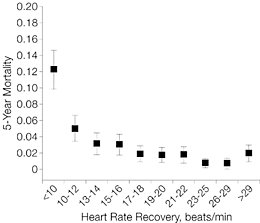
\includegraphics[width=0.5\linewidth]{dissertation//dissImages/BackgroundHRR.png}
    \caption{Enter Caption}
    \label{fig:enter-label}
\end{figure}

\subsection{Theoretical Maximum Heart Rate}
\label{sec:backgroundmaxhr}

Theoretical maximum heart rate (HR\textsubscript{max}) describes the approximate plateau of heart rate when a person exercises at their highest intensity. It is often used clinically as the backbone of calculating exercise intensity and the strain on the heart of a patient. 

‘Age-predicted maximal heart rate in healthy subjects: The HUNT Fitness Study’ by \cite{NesHRmax} investigates the validity of various formulae for calculating a person’s HR\textsubscript{max}. It compares the following calculations:

\begin{itemize}
    \item The Traditional Method of calculating HR\textsubscript{max} proposed by \cite{foxHRmax}: $$HR_{max} = 220 - Age$$
    \item Tanaka formula \cite{TANAKAHRmax}: $$HR_{max} = 208 - (0.7 x Age)$$
    \item Gulati formula \cite{GulatiHRmax}: $$HR_{max} = 206 - (0.88 x Age)$$
\end{itemize}

As well as proposing and comparing a new regression equation: $HR_{max} = 211 - (0.64 x Age)$

The study found a clear decrease in HR\textsubscript{max} with an increase in the participant’s age. Some other covariates also impacted the HR\textsubscript{max} of a participant, such as body mass index (BMI) - where participants classed as obese (with a BMI ≥ 30) had a modestly decreased HR\textsubscript{max} compared to people in the overweight and normal weight groups. It did however find that the rate of decline in HR\textsubscript{max} by age was not significantly impacted by covariates such as smoking status, gender or physical activity status.

My application can use the proposed formula as an accurate way of estimating the user's HR\textsubscript{max} using their age. This will allow me to estimate workout intensity and represent this to the user.


\subsection{Smartwatch Application Development}
\label{sec:backgroundwatchdev}

Developing an application for a smartwatch can result in many challenges, as noted by \cite{RamezaniDevelopingWatch}. The paper ‘Developing a Smartwatch-Based Healthcare Application: Notes to Consider’ outlines a case study of developing an Android healthcare application on a smartwatch for remote monitoring of geriatric patients, discussing the main challenges and design insights in the process.

The study explores several challenges hindering them through their development process, with the most notable being:

\begin{itemize}
    \item \textbf{Battery Life} - Smartwatches often have limited battery life in comparison to other mobile devices. It is important to ensure my application limits its battery consumption wherever possible.
    \item \textbf{Application Termination} - Non-native Android applications are often terminated by the smartwatch’s operating system (OS) to preserve battery life, disrupting continuous monitoring. When developing my application, it was essential to ensure health monitoring services were operating as a foreground service to prevent the OS doze mode from interfering
    \item \textbf{User Interaction} - The smaller screens and interfaces of smartwatches can cause difficulty in user interactions. It was essential to ensure the design of interactions and navigation throughout the apps was simple and intuitive to prevent user frustration
    \item \textbf{Sensor Configuration} - Personalising the collection and processing of sensor data for different individuals can be a complex task, ensuring correct calculations are carried out for each person. This is something I had to take into consideration when designing the profile building within the application and how the stored user data can be used to assist the accuracy of calculations
\end{itemize}


\section{Related Applications}
\label{sec:relatedapps}

\subsection{Fitbit}
\label{sec:fitbit}

Fitbit was a pioneer in the fitness-tracking community, boasting 40\% of the wearable devices market share in 2017 according to \cite{MarketShare2023}. However, more recently Fitbit have seen a major decline in their worldwide shipments in comparison to previous years. \cite{Fitbit2024} reported a 13\% decrease in their global unit sales in 2022 compared with the previous year. Notably, the company’s revenue is also taking a hit, with a 4.1\% decrease in the same period. However with 120 million registered users and 37 million reportedly using the app at least once a week, it still maintains its fair share of the market.

Fitbit devices have a similar heart rate monitor as found in most wearable devices, known as an optical heart rate sensor. This matched with the timekeeping functionality means it has all of the capabilities of calculating a user’s heart rate recovery however, it is still a major health-indicating feature it lacks. This has led to user dissatisfaction, as noted in this Fitbit community post from 2023 stating “Still looking for this feature in 2023. now I need to pay for an external app to view the data that Fitbit already has…for a fitness tracker this is a joke” \cite{FitbitReview}. This shows a clear gap for an application tailored towards automatic heart rate recovery measurements. Users want an intuitive and straightforward way for users to find their heart rate recovery and take important steps to manage their health based on the data presented.

\subsection{Apple Watch - HealthKit Repository}
\label{sec:applewatch}

Since the successful launch of the Apple Watch in 2015, Apple has consistently been a major player in the smartwatch market. According to \cite{MarketShare2024}, it has consistently been the top-selling individual vendor quarterly from 2018 through to Q3 of 2023, with the device sales continuously topping 20\% of global smartwatch shipments. While the Apple Watch is more tailored as a smartwatch than a fitness tracker, 92\% of smartwatch users are reported to use a smartwatch to track and maintain health and fitness, with 88\% stating it assisted in achieving fitness goals.

Apple Watch’s native workout and heart rate app are responsible for user fitness tracking and heart rate tracking respectively, all part of the Apple HealthKit repository. The Apple Watch does track the user’s heart rate recovery however, it cannot display historical records of heart rate recovery on the watch itself. HRR measurements are only available for the user to view on their watch on the day they complete their workout. The mobile ‘Fitness’ app does provide a historical record of data, however lacks a result comparison feature. The HRR graph presented by the app is very basic and provides no feedback as to what a user’s result means for their health. More than anything, it is very complicated to find this HRR information for a previous workout, with it being stated as “a lesser-known health metric that’s tracked by Apple Watch”, \cite{AppleHRR}

\begin{figure}[h!]
    \centering
    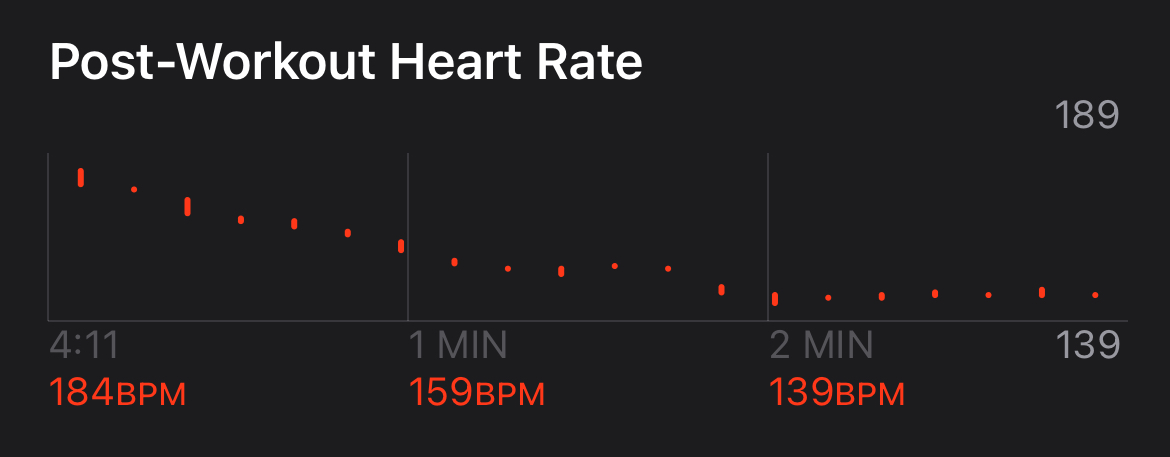
\includegraphics[width=0.5\linewidth]{dissertation//dissImages/AppleWatchHRR.png}
    \caption{Enter Caption}
    \label{fig:enter-label}
\end{figure}

This presents a clear opportunity to build an application that maintains the automatic HRR tracking of the Apple Watch while also adding some key missing features, notably:

\begin{itemize}
    \item Historical view of HRR
    \item Comparison of HRR measurements
    \item Explanation of what a user’s HRR means for them
\end{itemize}

%==================================================================================================================================
\chapter{Requirement Analysis}
\label{sec:requirements}

This chapter introduces the requirements the application must satisfy to be classed as successful. The requirements were gathered through weekly meetings with my supervisor Dr Sharon Ding. Throughout the project, we maintained an agile approach to the requirements where each meeting the progress and challenges were reviewed and minor adjustments to requirements could be made. The final requirements were then categorised into “Functional” and “Non-Functional” requirements as follows

\section{Functional Requirements}
\label{sec:functionalreqs}

Functional requirements define the features desired by end users. Prioritisation of these requirements is essential to ensure the development of the application is successful in such a short timeframe. I utilised the MoSCoW requirement prioritisation method (SOURCE), which involves separating the requirements into 4 categories:

\begin{itemize}
    \item Must Have 
    \item Should Have
    \item Could Have
    \item Will Not Have
\end{itemize}

\subsection{Must Have}
\label{sec:musthave}

"Must Have" requirements specify the essential features for the application's functionality:

\begin{itemize}
    \item \textbf{Heart Rate Tracking} - The application must be able to track a user's heart rate
    \item \textbf{Heart Rate Recovery Calculation} - The application must calculate the user's Heart Rate Recovery
    \item \textbf{Historic HRR Views} - The user must have some way to see their previous Heart Rate Recovery measurements
    \item \textbf{Visual Representation of HRR Readings} - The user must be able to visualise their Heart Rate Recovery
\end{itemize}

\subsection{Should Have}
\label{sec:shouldhave}

"Should Have" requirements specify important but not necessary features. These features still however add significant value:

\begin{itemize}
    \item \textbf{Fitness Tracking} - The application should allow for some form of fitness tracking
    \item \textbf{Automatic HRR tracking throughout a workout} - The application should automatically track a user's HRR throughout a workout
    \item \textbf{Feedback on what results mean for a user} - The application should give some form of feedback based on how good a HRR result is
    \item \textbf{HRR Comparisons} - The application should allow for a direct comparison between two HRR measurements to be made 
    
\end{itemize}

\subsection{Could Have}
\label{sec:couldhave}

"Could Have" requirements are features that could slightly add to the overall user experience, but are not massively important:

\begin{itemize}
    \item \textbf{Fitness History} - The application could store historical fitness statistics for the user to review
    \item \textbf{User Profile} - The application could have some form of profile building for a user
\end{itemize}

\subsection{Will Not Have}
\label{sec:willnothave}

"Will Not Have" requirements are features that might improve the overall user experience, but are not a priority for the given time frame:

\begin{itemize}
    \item \textbf{Support a variety of workouts} - In future, the application might host a variety of workouts to track.
    \item \textbf{Colour categorisation for multiple workout types} - In future, the application might have different colour schemes for different workout types.
    \item \textbf{Web Server for storing results} - In future, the application might store information on a web server to allow for viewing results on multiple devices.
    \item \textbf{Mobile App/Mobile-first Web App} - In future, the application might have a mobile/web application developed alongside to allow for additional functionality.
    \item \textbf{Goal Setting for workouts} - In future, the application might have a goal setting functionality, allowing users to set a goal to achieve in their chosen workout. For example, setting that they want to run 5 kilometres before finishing.
\end{itemize}

\section{Non-Functional Requirements}
\label{sec:nonfunctionalreqs}

Non-functional requirements focus on the quality of the finished product, ensuring practicality in the real world. These include:

\textbf{Performance} - The application is being developed on a smartwatch, meaning the performance of the application will be hindered by the smaller computational power in a smartwatch compared to a larger device such as a phone or a computer. It is important to ensure the finished product performs fluently with minimal latency across the system.

\textbf{Portability} -  The application will be used primarily while on the move, such as during an exercise. This means the application needs to be as easy as possible to view and interact with on the move. This is a common design issue when developing applications on a smartwatch (TICWEAR DESIGN SOURCE)

\textbf{Accuracy} - The application is attempting to give an insight into users' health based on their Heart Rate Recovery. If the values presented to the user are inaccurate it could lead to misleading or harmful information for the user

\textbf{Reliability} - It is also important the application is reliable. The previously mentioned “Should Have” category discussed users being able to compare HRR readings. Similar to the reasoning above, if the values over time are vastly different it could lead to harmful interpretations from the user.

%==================================================================================================================================
\chapter{Design}
\label{sec:design}

For some users this could be their first experience using a smartwatch application, therefore it was essential to design the application to be as intuitive as possible. 

There were four main considerations when approaching the user interface that will be discussed further:

\begin{itemize}
    \item \textbf{Application Flow Design} - Exploring the design of user flows throughout the application.
    \item \textbf{User Interface} - Discussing the initial prototyping of the user interface, including how users will interact and navigate through the application.
    \item \textbf{System Architecture} - Exploring the design of the chosen system architecture for the project
    \item \textbf{Database Design} - Explaining the structure, entities and relationships of the database
\end{itemize}

\section{Application Flow Design}
\label{sec:appflow}

A key aspect to consider when developing the application was how a user would go from opening the application to viewing a HRR reading. The flow of the application was a key factor to understand before starting development. The application has three main flows for the user to take, each accessible from the Home Page seen when the user launches the application as seen below.

The first and main application flow is to record a workout and measure the user’s HRR. This begins with the user selecting the workout they want to do - currently this is just running however, this is where the opportunity for additional workout options would be as discussed in section \ref{sec:futurework}. The application will then enter a multiple-page “Active Workout” display, consisting of two pages that can be swiped between. One page will display the current workout metrics, while the other page acts as a settings page with options to pause or end the workout. Selecting to end the workout then takes the user to another multiple-page “Post-Workout” display. Here the user will be able to see information about their heart rate recovery, heart rate, and more generic workout metrics, as well as being able to return to the home page. This can be visualised in a flow chart, displayed in Figure 4.1 below.



The application also has to allow users to view their previous HRR measurements as defined in the Must Have requirements in section \ref{sec:musthave}. This is accomplished by clicking the “Health History” button. The app navigates to a multiple-page health history display where all the user’s workouts are shown. Clicking on one of these workouts will then allow you to view the same three pages as the post-workout section in the workout flow, with the possibility for multiple HRRs to be shown. This flow can be seen in Figure 4.2 below.



Finally, the application also has a settings flow to allow for database modification. Accessible by clicking the settings icon on the home page, the application navigates to allow a choice between deleting workouts or viewing the set-up profile. If the user selects delete workouts, all workouts stored on the watch are deleted. Otherwise, clicking view profile will display the currently stored user information. This can either be edited - where the user passes through the profile builder described more in section \ref{sec:usersettings} to modify the database - or deleted - deleting the stored user from the database and navigating to set up a new profile. This can be seen in Figure 4.3 below.

\section{User Interface}
\label{sec:ui}

When initially approaching the challenge of developing prototype designs, I developed wireframes on Figma. Figma is a very useful tool for developing wireframes quickly by sketching a rough idea of how the application was going to look, with the added ability of creating user interactions. However, it was agreed upon early between me and my supervisor - Dr Sharon Ding - that it would be more beneficial to develop the design directly on the smartwatch itself. This would allow the testing of the user interaction alongside the design to ensure intuitiveness and clarity. It also gave me a more accurate scale to work on when developing the design, rather than developing on a much larger monitor. This also meant the design was one of the key focuses of the evaluation process, discussed further in section \ref{sec:userstudyaims}.

To discuss the final design I’ll break down the application into the three separate flows, discussed earlier in section \ref{sec:appflow}. 

\subsection{Active Workout}
\label{sec:activeworkout}

The active workout flow consists of six main pages, being:

\begin{itemize}
    \item \textbf{Select a Workout} - A basic page with buttons allowing the user to select a workout type. Currently this only displays running, however as explained in \ref{sec:futurework} this is where other workout types would be added.
    \item \textbf{Active Workout Page} - The page users see while tracking a workout. This page design is discussed further below \ref{sec:activeworkoutsubsection}.
    \item \textbf{HRR Measurement in Progress} - A timed page that shows the user their progress during a HRR reading. The circular design of this page is inspired by \cite{TicDesign}
    \item \textbf{HRR Measurement} - The page a user sees 60 seconds after ending their workout. It shows the user a graph representation of their Heart Rate Recovery, discussed further in section \ref{sec:hrrgraph}
    \item \textbf{Heart Rate Range} -  A page showing the user their heart rate across the span of their workout. The graph design and implementation are discussed further in \ref{sec:hrrangegraph}
    \item \textbf{Workout Metrics} - A simple page giving users other information from their workout, such as calories burned, active time and more. It’s also key navigationally for allowing users to return to the home page once their workout is complete.
\end{itemize}

\begin{figure}[h!]
    \centering
    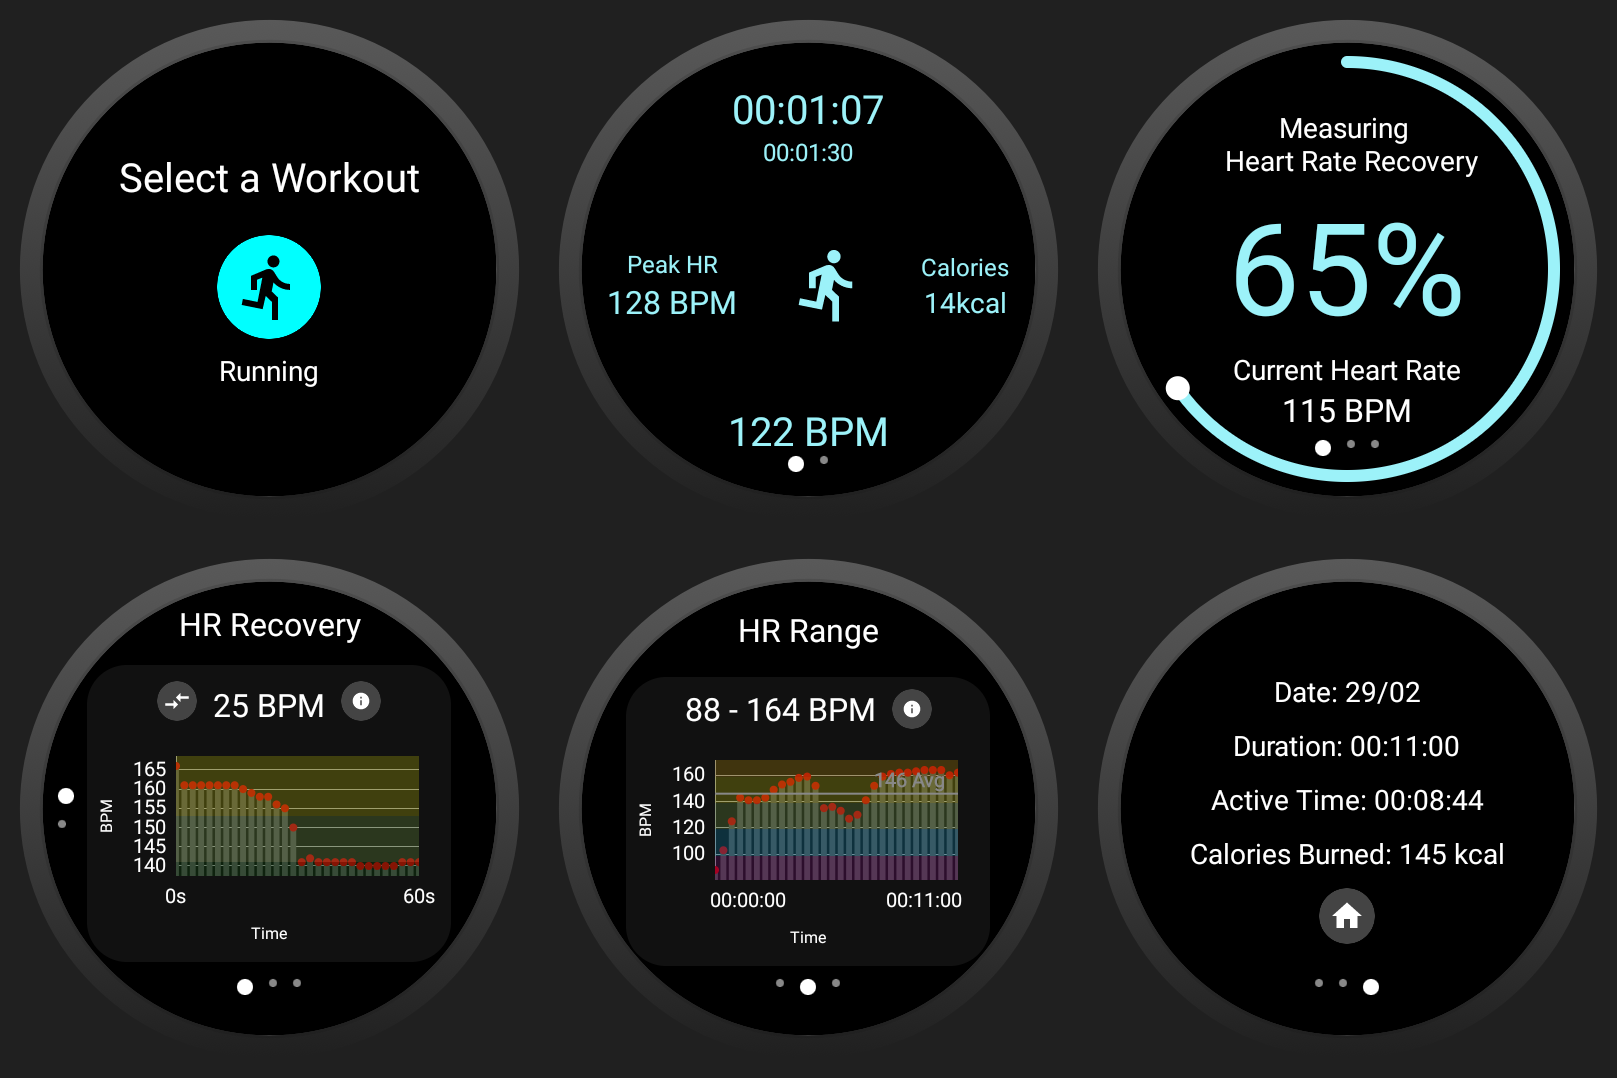
\includegraphics[width=1\linewidth]{dissertation//dissImages/ActiveWorkoutCombined.png}
    \caption{Enter Caption}
    \label{fig:enter-label}
\end{figure}

\noindent\mbox{}\\
\subsubsection{Active Workout Page}
\label{sec:activeworkoutsubsection}
\noindent\mbox{}\\


Upon users selecting their workout, they are met with the Active Workout page. The design for this page was a statistic-focused approach, giving the user as much information as possible without over-cluttering the screen. The workout was separated into five sections:

\begin{itemize}
    \item Two timers at the top of the screen that show users their active moving time and total workout duration.
    \item The user’s peak heart rate throughout their workout is shown on the left.
    \item An icon in the centre show the user what type of workout they are tracking, in the case of my prototype this is always going to be running
    \item An active calorie tracker on the right shows how many calories the user burned during their workout
    \item The user’s current heart rate, displayed at the bottom of the screen
\end{itemize}

There is also a progress bar surrounding the display, showing a user how close they are to completing a goal they set before the workout such as a target distance or time.

The user can interact with this page through the horizontal pagination of the application, allowing users to swipe along to reveal the workout settings. This workout settings page is a simple page consisting of a play/pause button and an end workout button. The circles seen at the bottom of the design give users a prompt that more content is available than what the initial active workout page shows, according to \cite{PageIndicators}. 

\subsection{Health History}
\label{sec:healthhistory}

The health history flow also consists of six pages, with two of these being nearly identical to some pages described above:

\begin{itemize}
    \item \textbf{Select a Workout} - This allows users to select a database-stored workout to review. This is set up with a horizontal pagination to show two workouts per page, with circles acting as a page indicator at the bottom to give context to the user of the number of workouts stored. Each workout shows the date the workout was completed below so users can understand what each workout is.
    \item \textbf{HRR Measurement} - The design of this page is identical to the design seen on the active workout page, however has a few navigational differences. This page allows users to view all of their HRR readings recorded during the workout if any more have been taken. The graph also has a “Compare” icon in the top left, where selecting this opens the HRR Select page for users to compare results. This is done to accomplish “HRR Comparisons” discussed as a Should Have requirement in section \ref{sec:shouldhave}
    \item \textbf{Heart Rate Range} - This page is entirely identical to the Heart Rate Range page displayed to the user at the end of a workout, described in section \ref{sec:hrrangegraph}
    \item \textbf{Workout Metrics} - Similarly this design is also identical to the page described above, with the only slight navigational difference being the home button navigates to the Select a Workout Page rather than the application home page.
    \item \textbf{HRR Select Compare Page} - This page is designed similarly to the Select a Workout Page, however contains the HRR measurements in the buttons themselves to give users more context on what the measurement they are comparing the result against was like.
    \item \textbf{HRR Compare} - The comparison page shows two different HRR measurements plotted on a graph for easy comparison. The specific design and implementation of the graph are discussed more in section \ref{sec:hrrcomparison}. This page uses horizontal pagination once again, allowing users to swipe across to view each of the results individually with the same design as the HRR measurement described in the previous section, finishing with a return to compare button that allows users to return to the  HRR Select Compare Page
\end{itemize}

\begin{figure}[h!]
    \centering
    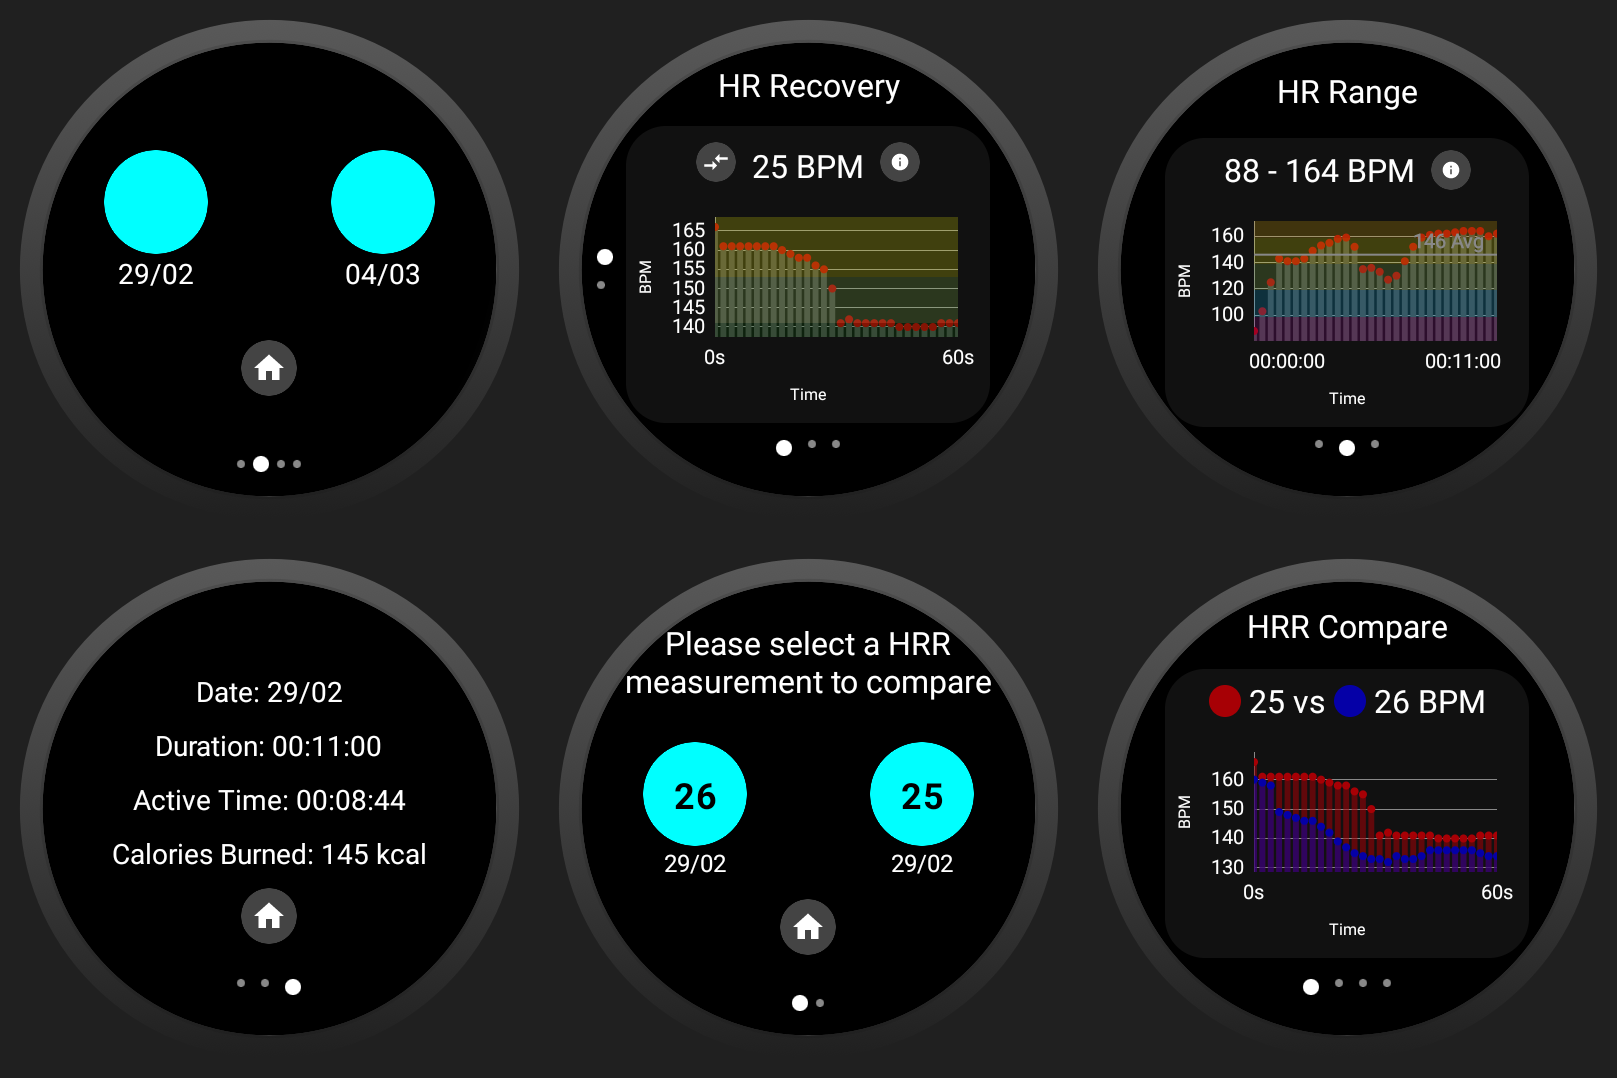
\includegraphics[width=1\linewidth]{dissertation//dissImages/HealthHistoryCombined.png}
    \caption{Enter Caption}
    \label{fig:enter-label}
\end{figure}

\subsection{User Settings}
\label{sec:usersettings}

The user settings flow contains seven pages, with a few of these pages being very similar in design to one another:

\begin{itemize}
    \item \textbf{User Settings Page} - The landing page when a user enters the user settings flow. It is designed with a simple display of two buttons, one for viewing the profile and one for deleting the workout. The colours are plain here to prevent a user from doing an unintentional and irreversible action, such as a database deletion
    \item \textbf{Profile View Page} - This page displays the stored information about the user: their age, weight and gender. This is displayed as a list at the top of the page to make it easy for users to see if their information is correct.
    \item \textbf{Are You Sure Page} - This page asks the user if they are sure they want to continue with their action, with a simple ‘Yes’ button - with a tick icon - or ‘No’ button - with a cross icon. This layout was chosen to keep consistent with existing technologies. There are two different versions of this page with identical designs that pose different questions - one for deleting workouts and one for deleting profiles.
    \item \textbf{Enter Birthday Page} - Here users can enter their birthday to be used for calculating their age at a later stage. Having the user enter their birthday rather than their age directly means the application can automatically update the user’s age rather than requiring them to change it every year. This page is designed with three buttons arranged horizontally, labelled “Day”, “Month” and “Year” respectively. Each of these buttons is associated with a drop-down menu that allows users to select a date. Finally, there is a green button at the bottom with a tick icon, indicating to the user to confirm their choice with this button once they have entered their birthday.
    \item \textbf{Enter Weight Page} - This page allows users to enter their weight. The design is inspired by the Enter Birthday Page to keep consistency across the profile-building process. The page has a button linked to a drop-down menu in the centre of the screen, showing the scale of “kg” next to it. Finally, the same green tick button is at the bottom, allowing users to confirm their selection once they have entered their weight.
    \item \textbf{Select Gender Page} - Here users can select their gender, choosing between “Male”, “Female” or “Other”. The buttons contain the respective icons for each of the genders. When a user selects one of the buttons it inverts the colours, highlighting the selected choice. The consistent design across the profile building is then maintained, with the green tick button in the same position at the bottom of the screen to confirm the choice.
    \item \textbf{Successfully Deleted Page} - A basic splash screen that displays for 2 seconds, showing the user a confirmation message that the deletion was successful - either “Profile Successfully Deleted!” or “Workouts Successfully Deleted!”
\end{itemize}

\begin{figure}[h!]
    \centering
    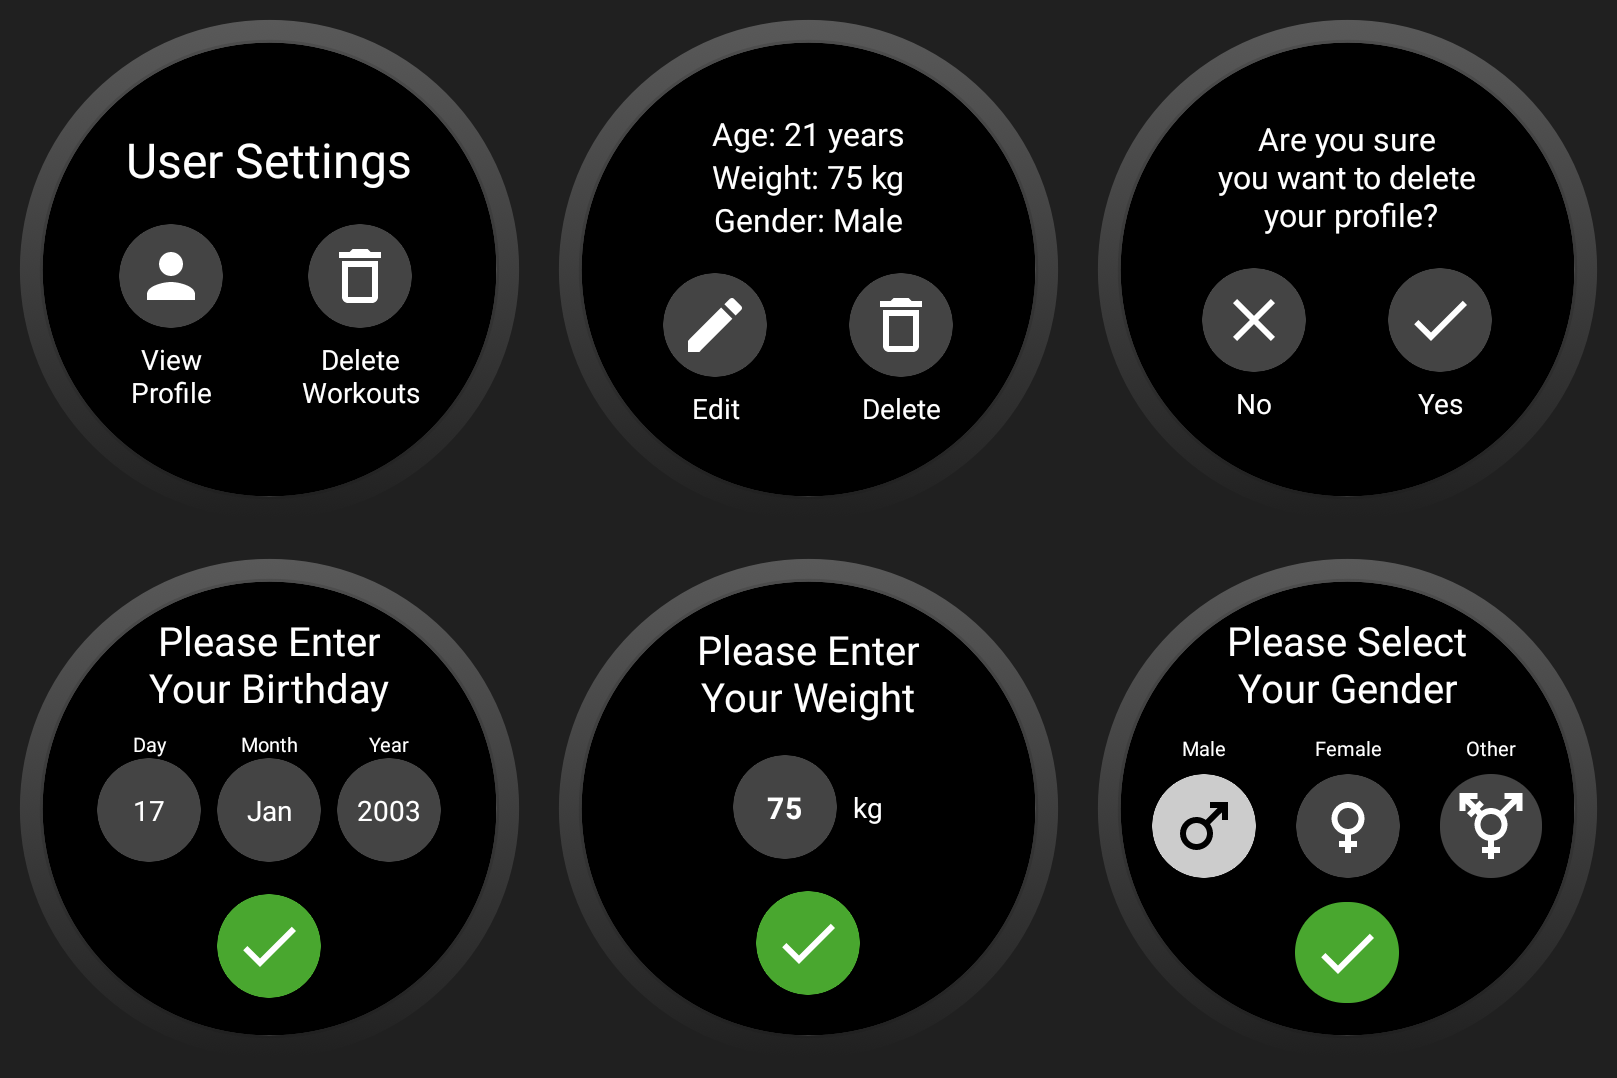
\includegraphics[width=1\linewidth]{dissertation//dissImages/UserSettingsCombined.png}
    \caption{Enter Caption}
    \label{fig:enter-label}
\end{figure}

\section{System Architecture}
\label{sec:systemarch}

The application is structured around the Model-View-ViewModel (MVVM) architecture, containing three core components:

\begin{itemize}
    \item \textbf{Model} - This layer represents the core data structures, including sensor data gathered. It is also responsible for retrieving and updating data from the database.
    \item \textbf{View} - This layer presents the UI to the user, modified by the ViewModel layer
    \item \textbf{ViewModel} - This serves as an intermediatory layer between the View and the Model, retrieving information from the Model and presenting it to the View to update the UI accordingly. It contains classes that handle data and perform calculations, as well as handling sensor management.
\end{itemize}

\section{Database Design}
\label{sec:databasedesign}

The project database has a simple design, with only two entities required for the implementation:

\begin{itemize}
    \item A \textbf{“User”} object - holding all of the information about the user required for calculations
    \item A \textbf{“Workout”} object - holding all of the information regarding workout length, date, and heart rate information throughout the workout
\end{itemize}

The relation of these objects does not require foreign keys in the database design. This is because there can only ever be one user object that all workout objects are inherently related to. It was still however important to have unique identifiers for each of the objects, being the primary keys of the entities. For the User object, this identifier is a name field, which is always set to “user” for referencing later. For the Workout object, the identifier is an auto-incrementing ID number.

\begin{figure}[h]
    \centering
    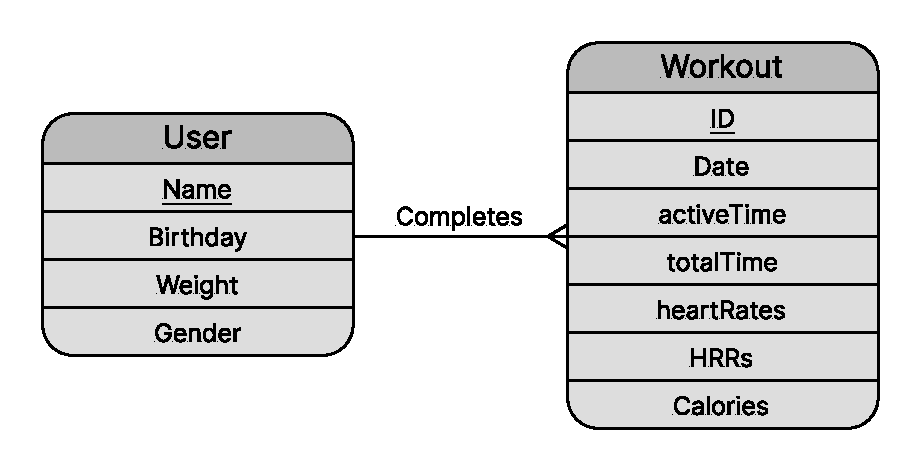
\includegraphics[width=0.75\linewidth]{dissertation//dissImages/ERDiagram.pdf}
    \caption{Enter Caption}
    \label{fig:enter-label}
\end{figure}

%==================================================================================================================================
\chapter{Implementation}
\label{sec:implementation}

This chapter describes the implementation methods and techniques used throughout the development of the application. It discusses the hardware and software configuration for development, before discussing the algorithms implemented and concluding with the data visualisations displayed to users.

\section{Development Environment}
\label{sec:devenv}

Development for this project was carried out on the Mobvoi TicWatch Pro 3 GPS, an Android-based smartwatch with the Google Wear OS operating system. The smartwatch includes several sensors accessible through simple API calls built into Android, allowing me to interact freely with the Heart Rate Monitor and Accelerometer as discussed in later sections. 

Application development was carried out on Android 9 “Pie”, corresponding to Wear OS 2.26. Later through the evaluation process, an updated version of Android was tested also ensuring the app remained fully functional on Android 11 “R” with Wear OS 3.5.

The IDE used for the project was Android Studio, the official IDE for Android development built by JetBrains as an extension from IntelliJ. Android Studio has many great features out of the box that ease development, such as the ability to run device emulators to see changes and debug issues quickly without having to download the application to the watch, as well as real-time linting and quick fixes to help spot mistakes or redundancies in code. Another major benefit of developing on Android Studio was the built-in Android Debug Bridge (ADB) - part of the Android Software Development Kit (SDK) - that allows Android Studio to directly connect to the TicWatch over WiFi to send application packages to the watch to be installed.

\section{Technologies}
\label{sec:technologies}

When deciding on technologies, there were three main areas of concern:

\begin{itemize}
    \item A well-documented and modern programming language to develop the application
    \item A reliable and robust layout framework to make the application as user-friendly as possible
    \item A synchronous and efficient database structure to store data
\end{itemize}

In this section, I will explore the different considerations when selecting the chosen technologies. This includes a brief history of the various technologies, before moving on to the standout features that prompted me to use them and the drawbacks I remained aware of while developing with them

\subsection{Kotlin vs Java}
\label{sec:kotlinvsjava}

Historically, Android apps have primarily been developed in Java, the official language of Android Development since Android’s inception in 2008. However, since the release of Kotlin more and more developers have made the change over from Java for feature development.

Kotlin is a statically typed, high-level programming language officially released in 2016 by JetBrains, the company behind the popular Integrated Development Environments (IDEs) IntelliJ and PyCharm (SOURCE). Kotlin was developed with the idea it would become a “better language” than Java ([SOURCE](https://www.jrebel.com/blog)). It remains a younger programming language compared to similar long-term languages such as Java however, was already announced as the preferred programming language for Android development by Google at the Google I/O Conference in 2019.

Kotlin is strongly influenced by Java syntactically while simplifying some of Java’s constructs such as semicolons to end a statement and getter and setter methods. The concise nature of Kotlin - through features such as type inference - allows for around 20\% less code to provide more functionality according to Medium ([SOURCE](https://medium.com/@johnkorly/kotlin-vs-java-performance-drill-down-which-to-choose-2514bdf91916)). Another key benefit of choosing Kotlin is reliability. Due to the nature of static types and null checking in Kotlin, it is reported that Google Home saw a 33\% decrease in NullPointerExceptions after changing over development to Kotlin, with the top 1,000 apps on the Google Play Store having 20\% fewer crashes per user on average ([SOURCE](https://medium.com/androiddevelopers/fewer-crashes-and-more-stability-with-kotlin-b606c6a6ac04)). Ultimately, Kotlin is now the chosen development language by several major international companies such as Netflix, Slack and X due to its benefits over Java however, that doesn’t mean Kotlin doesn’t have its drawbacks.

One of the main difficulties I was wary of was the age of the language. As previously mentioned Kotlin was first stably released in February 2016, just over 20 years after the first Java release in 1996. This immaturity in comparison to Java causes less documentation and general community when trying to solve a problem. In general, when finding a bug in your code you are much more likely to find a solution developing in Java compared to Kotlin. FIND ANOTHER NEGATIVE POINT TO BOOST THIS LAST PARAGRAPH

\subsection{Jetpack Compose vs XML}
\label{sec:composevsxml}

Android user interface (UI) development has undergone several changes and improvements over the years. Initially, it was standard to build UIs with XML, a markup language that defines the layout and appearance of UI elements. Using XML allowed developers to separate the layout from the logic of the application and reuse whole components made of XML, similar to many popular modern Web Application frameworks such as React and Flutter. However, XML also had several drawbacks such as its verbosity and inability to support dynamic changing UIs that change for different events. In 2019, Google announced their experiment to solve some of these issues through a project named Jetpack Compose.  It was further refined across two years before reaching its first stable release in July 2021. Since then it has evolved into the recommended way to build Android UI by Google.

Jetpack Compose is a “modern UI toolkit” that aims to simplify the UI development process in Android. It allows for all the functionality of XML and more while maintaining the conciseness of Kotlin programming. In 2020 (CHECK THIS), the TV show tracking Android application ‘Tivi’ went through a migration of an XML-based layout approach to Jetpack Compose and saw a 41\% decrease in Android Package (APK) when using Jetpack Compose. They also report a 76\% decrease in XML lines as well as an 8\% decrease in Kotlin lines across the project while maintaining a very similar application layout. Finally, they also found a 29\% reduction in build time after converting the project to Jetpack Compose. Moving away from statistical improvements, Jetpack Compose also easily allows for dynamic rendering through the use of states. With all the performance improvement and concise nature of Jetpack Compose, alongside the dynamic rendering necessary for my application, Jetpack Compose was the clear choice

However, Jetpack Compose isn’t without its challenges and difficulties. Regardless of the layout framework chosen - XML or Jetpack Compose - they were both new frameworks however, XML is much more similar to previous layout technologies I’ve used such as HTML and CSS. This likely required a slightly longer time to practice and master Jetpack Compose than if I chose to develop in XML. This learning curve is worsened by the lack of documentation and resources available in comparison to XML ([SOURCE](https://medium.com/@gaga.lomidze/xml-vs-jetpack-compose-advantages-and-disadvantages-538ceee28dbd)) due to how new the framework is.

\subsection{Room Database}
\label{sec:room}

Android development has always relied on SQLite - a lightweight and efficient relational database management system - for applications storing data. It is a powerful tool that is well-suited for small to medium-scale projects, known for being reliable and efficient. However, dealing directly with SQLite can be complicated, relying on a lot of boilerplate code to work effectively (SOURCE).

The Room Database is an Android library that simplifies data persistence (SOURCE). It is used as a layer of abstraction over SQLite, maintaining efficiency while reducing the complexity of database interactions. Room is an Object Relational Mapping (ORM) library, meaning it maps database objects directly to Java objects to be interacted with in our code. This greatly reduces the need for boilerplate code when developing a database system. 

Room also has the added benefit of built-in compile-time SQL validation. This means that Room ensures the SQL operations throughout the application are valid, rather than having to debug a crash that would be standard with using an SQLite approach.

Room has three main components:

\begin{itemize}
    \item \textbf{Entity} - An Entity as the name suggests represents an entity in the database. In my application, there are two entities used - a ‘User’ and a ‘Workout’ entity. This is responsible for defining the data types and the structure of the object, allowing for convenient reading and manipulation by Kotlin code when necessary
    \item \textbf{Data Access Object (DAO)} - DAOs are responsible for the interactions with the database. It translates functions called in the Kotlin code into SQL requests, allowing for efficient access to the database whenever it is required
    \item \textbf{Database} - The Database object holds the actual database, and is responsible for instantiating the database upon the launch of the application. It is the main part of the component stack allowing for data persistence, even when the application is closed or the device powers off
\end{itemize}

\begin{figure}[h]
    \centering
    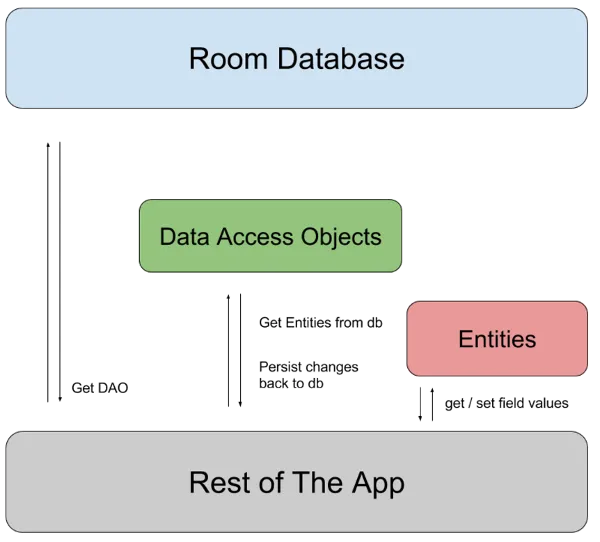
\includegraphics[width=0.5\linewidth]{dissertation//dissImages/RoomDatabaseStructure.png}
    \caption{Enter Caption}
    \label{fig:enter-label}
\end{figure}

\section{Algorithms}
\label{sec:algorithms}

Algorithms are the backbone of functionality within my application, processing and reacting to data to calculate and present detailed results to the user. This chapter will investigate the three algorithms imperative to functionality:

\begin{itemize}
    \item \textbf{Heart Rate Recovery Algorithm} - The core algorithm that, when called upon, stores and calculates the change in a user’s heart rate across a minute. The algorithm stores these heart rates as a list in the database to be used in the results section
    \item \textbf{Automatic Pausing/Automatic HRR Algorithm} - An algorithm essential for the functionality of measuring HRR during a workout. This allows for the detection of a break in the workout, where if this break is greater than a minute in length an extra HRR reading can be taken automatically.
    \item \textbf{Calorific Expenditure Algorithm} - An algorithm used to track the calories burned by the user during a workout. Another useful health metric based on age, weight, gender and heart rate that further helps a user understand how intense their exercise was.
\end{itemize}

These algorithms were implemented in an Android ViewModel as previously discussed in chapter (ENTER CHAPTER HERE) so the calculations can happen in the background and do not prevent the user from using and navigating the application.

There are a few other processes reliant on these algorithms not further explained, one of which is the updating of the progress variable. This progress variable is a measure of the completion percentage of a HRR reading, stored as a floating point number and updated throughout the HRR algorithm. The progress is used during the results section, described in section (ENTER CHAPTER NUMBER HERE), and allows for a progress-bar style update to the user to visualise how far through their HRR reading they are.

The Automatic Pausing functionality described in the automating HRR measurements subsection describes setting the application state to paused or resumed depending on the movement of the device. This application state determines the difference between the Active Time - the time a user is actively moving for - and the Total Duration of a workout - the total time since the workout started. This allows a user to get a more accurate understanding of how long they have been working out.

Finally, the application makes use of theoretical maximum heart rate. This is determined by (SOURCE) as a reliable method to approximate the maximum heart rate of the user, based on their age. It is implemented with the following function:

$$
MaxHR = 211 - (0.64 \times A)
$$

Where $A$ is the user’s age.

\subsection{Heart Rate Recovery}
\label{sec:hrrimplementation}

The main algorithm the application is built around is the Heart Rate Recovery algorithm. This is handled in the form of a function that, when called upon, will track the user’s heart rate over the space of a minute and return the list of results. The reasoning behind returning a list of results is so heart rates can be plotted in a smooth bar chart for the user to help visualise this change in heart rate. This algorithm is run asynchronously to maintain app usability and navigation while these measurements and calculations are happening. 

The algorithm is dependent on the heart rate sensor, another function implemented in the ViewModel. The function registers a listener to the heart rate sensor and then detects any updates from the heart rate sensor. It also keeps track of the peak heart rate that can be used in the HRR calculation, as described in step 1 below. 

To breakdown the algorithm, these are the steps that happen once the function is called:

\begin{enumerate}
    \item All variables are initialised. This includes setting the progress variable to 0 and adding the user’s maximum heart rate to the HRR heart rate list as the beginning heart rate.
    \item Then comes a supposedly infinite while loop with a few break conditions:
    \begin{itemize}
        \item If the loop has been running for greater than or equal to 60 seconds then break from the while loop
        \item If user movement has been detected during a HRR reading then reset all variables changed and break out of the function entirely
    \end{itemize}
    This loop is repeated every 10 milliseconds to update the progress variable smoothly
    \item During these 60 seconds, heart rate values are added to a new temporary list every 10 milliseconds. Once this list has reached 25 elements in length, the average of these values is added to the bigger HRR heart rate list and the temporary list is reset. This allows for one heart rate to be stored every 250 milliseconds. I found this to be a good balance of capturing variance in the sensor data without overwhelming the database by storing excessive data
    \item After 60 seconds have elapsed the HRR heart rate list holds the values from the reading. The separating value ‘-1’ is added to the list to be used as a separating value, due to the impossibility of -1 ever appearing in the data itself. The peak heart rate is reset to 0 to be used for the next reading.
    \item Finally, the workout object is updated in the database to reflect this new HRR reading. This is done by collecting the most recent workout object, which will always be the current workout, and then appending the gathered data to the end of the list to maintain any previous readings.
\end{enumerate}

When the application requires individual HRR readings, the entire list of heart rates can be collected from the workout object. This list is then split with the -1 separators previously inserted, with each sub-list being a separate HRR reading. The list is passed into the graphing function to display to the user, with the actual HRR value being displayed as the first value stored in the list - being the user’s peak heart rate explained in step 1 - minus the final stored heart rate - being the user’s heart rate after one minute.


\subsection{Automating HRR Measurements}
\label{sec:autohrr}

The algorithm behind automating HRR measurements is an extension of the auto-pausing functionality, dependent on accelerometer data for movement detection. This functionality was implemented in such a way that whenever the user takes a break, the application will automatically detect this and - where the break extends the minute in length required for a HRR reading - will record a HRR reading in the background that can be reviewed at a later stage.

The movement detection algorithm is implemented as follows:

\begin{enumerate}
    \item Whenever the accelerometer sensor is updated - approximately every 10 milliseconds - the magnitude of the acceleration is calculated. This is done with the following formula:

    $$
    \sqrt{x^2 + y^2 + z^2} - 9.81
    $$
    
    Where $x$, $y$ and $z$ represent the three axes of direction. Note the subtraction of 9.81 is to counteract acceleration due to gravity
    \item The magnitude is then added to a measurement list. To keep this list to a standard size, whenever this list exceeds 300 readings, the first reading is removed. Due to the nature of a sensor updates approximately every 10 milliseconds, the measurement list stores approximately a 3-second window of acceleration magnitudes. The average of this list is then calculated, with this value representing the user’s movement across the 3 seconds.
    \item If this average acceleration value drops below the threshold value of 2.75, the application assumes the user to be taking a break. When this happens, the application triggers a vibration to indicate to the user the change in status. 
    \item The application then calculates the theoretical maximum heart rate (POTENTIAL FOR A SOURCE HERE) of the user. Then, ensuring the application is still in a paused state and the current heart rate is greater than half of the theoretical maximum for the user, the application triggers an intermediate HRR reading
\end{enumerate}

Both of the algorithm’s hyperparameters - the threshold value for stopping movement (at 2.75) and the number of readings stored at once from the accelerometer (at 300) - were tuned through the auto-ethnography, with further feedback to optimise the accuracy gathered through the pilot and user studies

\subsection{Calorific Expenditure Algorithm}
\label{sec:calories}

The final algorithm explained in detail is the calorific expenditure calculation, used to accumulate the calories burned during a workout. The algorithm heavily relies on the information provided by the user at the profile creation stage, including their weight, age and gender. This calculation is based on (ENTER SOURCE HERE).

The algorithm is implemented as follows:

\begin{enumerate}
    \item Upon a user starts a workout, the function for calculating calories is called. The algorithm acquires the user’s details from the database and calculates the user’s age from their birthday.
    \item Once the algorithm has the user’s details, it enters a while loop with the condition that the state variable calculateCalories is set to true. This state variable is initialised as true and only set to false once a user has finished their workout. Within this while loop, the calories burned across one second are calculated. There are three different calculations the application can use, depending on the gender selected by the user at the time of profile creation:
    \begin{itemize}
        \item Where the user has selected male, the following calculation is used ($H$ = Current Heart Rate, $W$ = User Weight, $A$ = User Age):
        $$
            \frac{-55.0969 + (0.6309 \times H) + (0.1988 \times W) + (0.2017 \times A)}{4.184 \times 60}
        $$
        \item Where the user has selected female, the following calculation is used ($H$ = Current Heart Rate, $W$ = User Weight, $A$ = User Age):
        $$
            \frac{-20.4022 + (0.4472 \times H) + (0.1263 \times W) + (0.074 \times A)}{4.184 \times 60}
        $$
        \item Where the user has selected other, the calculation is determined as the average of the results of the previous two equations. While this solution is not necessarily the most accurate method of measuring calories in this circumstance, according to ([Calculating TDEE/BMR for Transgender or Non-Binary Individuals – ABC Trainerize Help Center](https://help.trainerize.com/hc/en-us/articles/16950447732372-Calculating-TDEE-BMR-for-Transgender-or-Non-Binary-Individuals)) there is “currently no calculation or guideline that does not use sex assigned at birth” to do this calculation, therefore, I believed it to be the best solution to ensure my application caters to as many people as possible.
    \end{itemize}

    \item The result of this calculation is then added to a running total, with this running total being accessible to the frontend of the application to display to the user and store in the database upon workout completion. This while loop is repeated once a second to ensure frequent updates of the current calorie count.
    
\end{enumerate}


\section{Visualising Results}
\label{sec:visualiseresults}

To present HRR reading results to the user I used a graphical representation, with the main aim of this approach to allow users to visualise complex numbers as a clear and easy-to-understand graph. Tableau (https://www.tableau.com/data-insights/data-visualization/advantages-disadvantages) states that using graphs for data visualisation allows users to more easily comprehend results compared to just showing numbers, leading to a quicker absorption of knowledge.

There are three different categories of graphs implemented within my project, all implemented as bar charts:

\begin{itemize}
    \item \textbf{Heart Rate Recovery} - A representation of the user’s falling heart rate across a minute-long period
    \item \textbf{Heart Rate Range} - A representation of the user’s heart rate throughout their workout, plotted against the duration of their exercise
    \item \textbf{HRR Comparison} - A comparison graph that plots two Heart Rate Recovery measurements, chosen by the user, to display the difference between the two results.
\end{itemize}

The graphs were implemented using the MPAndroidChart library (LINK TO GITHUB HERE). I chose to use this graphing package due to its high level of customisability through a custom renderer. This renderer was implemented slightly differently for each of the graphs mentioned above. In general, it was used to give users more information than just a standard bar chart, where I could highlight target “zones” or differentiate two separate sets of results. MPAndroidChart graphs also have a built-in animation for rendering the bar charts, plotting the results chronologically to further emphasise the progression of readings. 

\subsection{Heart Rate Recovery Graph}
\label{sec:hrrgraph}

Heart Rate Recovery is the first graph a user sees after they complete a workout. To plot the graph, the first step involves a bucketing process, to normalise the HRR list provided into standardised 30 values. This is a necessary step to maintain the graph styling across the app regardless of the raw values stored in the database. It averages the readings across the graph and gives the user a good overview of how their heart rate varied over the minute-long period. 

To implement this, I first extracted the start and end values from the list, as these were key for calculating the actual heart rate recovery. Heart rate recovery is the peak heart rate minus the heart rate after a minute, therefore we want these exact values not to be impacted by the bucketing process. The rest of the values in the raw list are then processed to fill in the other 28 different values. The bucket size is calculated by dividing the length of the list minus the first and last values by 28, rounding down to the nearest whole number. The remainder is separated across the starting buckets until the index is the size of the remainder. Here is an example of how this works in practice, with a list size of 168 values:

\begin{itemize}
    \item Remove the first and last values of the HRR list for the first and last values in the graph
    \item Divide the remaining 166 by 28 = 5 with remainder of 26
    \item Bucket size of 6 for the first 26 buckets, and 5 for the remaining 2
    \item Take a sublist of the HRR list for the bucket, and add the average as a value to be plotted on the graph
\end{itemize}

Once the list has been normalised to 30 values through the bucketing process, the graph is then plotted. The x-axis shows the progress of time, showing 0s and 60s at the two ends of the measurement. The y-axis shows the heart rate values, allowing users to see the heart rate values throughout the measurement. Above the graph is the actual HRR value, calculated by subtracting the first and last heart rate stored in the HRR list.

\begin{figure}[h]
    \centering
    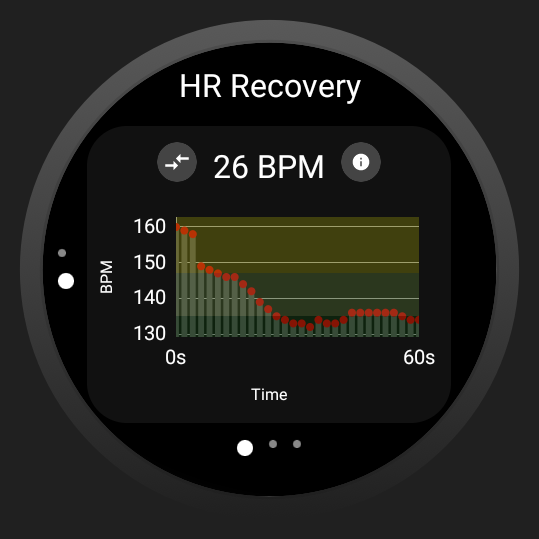
\includegraphics[width=0.5\linewidth]{dissertation//dissImages/HRRGraph.png}
    \caption{Enter Caption}
    \label{fig:enter-label}
\end{figure}

As well as the heart rates plotted on the graph, there are also some highlighted zones. These are used in both the Heart Rate Recovery and Heart Rate Range graphs to provide users with more information at a glance on how their readings compare to what is expected. In the case of HRR, there are three different zones:

\begin{itemize}
    \item \textbf{Zone 1 (Low HRR)} - This level indicates a recovery of less than 13 BPM, associated with poor fitness and athletic performance
    \item \textbf{Zone 2 (Healthy HRR)} - This level indicates a recovery between 13 and 25 BPM, associated with an overall average fitness and athletic performance
    \item \textbf{Zone 3 (High HRR)} - This level indicates a recovery greater than 25 BPM, associated with improved fitness and athletic performance
\end{itemize}

These zones are possible thanks to the custom renderer, mentioned in section \ref{sec:visualiseresults}. They are calculated and plotted synchronously with the rest of the graph, coloured semi-transparently to prevent the colours from over-cluttering the graph and confusing users. Users can understand what each of the zones indicates by clicking the information icon, located at the top-right of the graph. The values selected for Low, Healthy and High HRR are from the same paper mentioned in section \ref{sec:backgroundhrr}, \cite{HRR2000}.

\begin{figure}[h!]
    \centering
    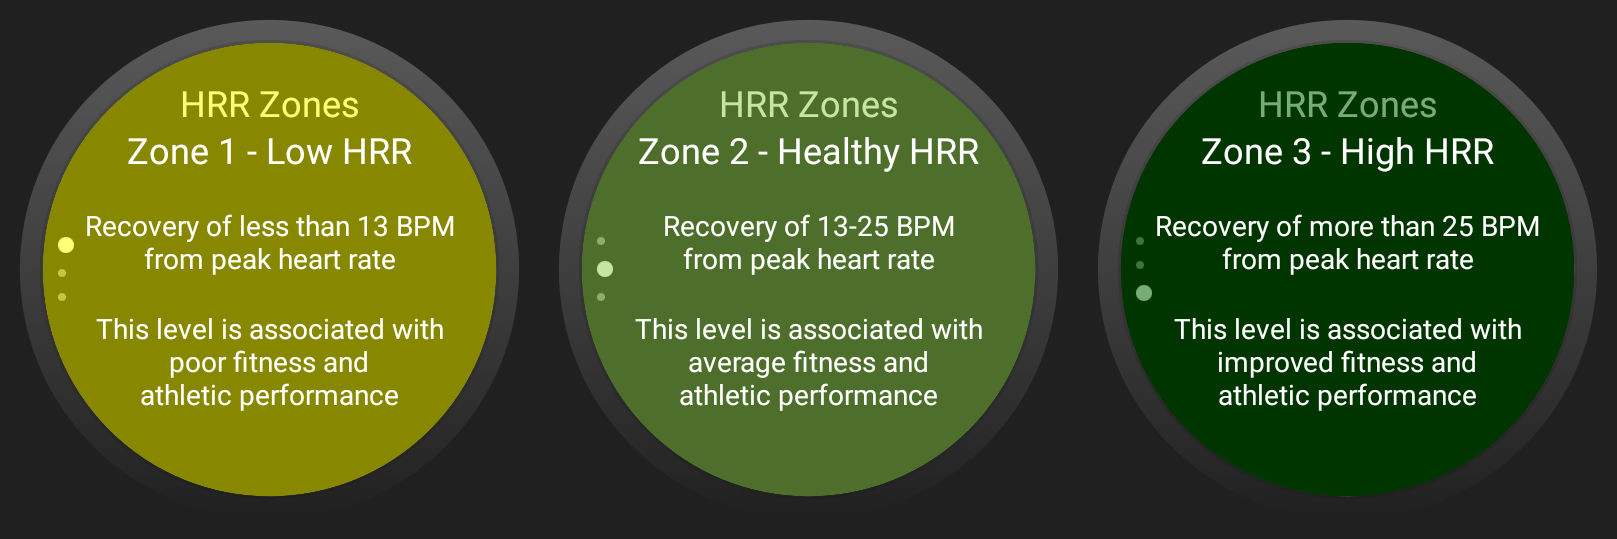
\includegraphics[width=1\linewidth]{dissertation//dissImages/CombinedHRRZones.png}
    \caption{Enter Caption}
    \label{fig:enter-label}
\end{figure}

At the top of the graph, there is also another icon top-left. This icon allows the user into the HRR Comparison page, discussed further in section \ref{sec:hrrcomparison}

\subsection{Heart Rate Range Graph}
\label{sec:hrrangegraph}

When swiping along from the HRR bar chart, you are met with another bar chat showing the Heart Rate of the user across their workout. The implementation of this graph begins in the same way as the HRR bar chart, where the long list of heart rates retrieved from the database is normalised into 30 average values representing the whole workout. This is achieved with an identical bucketing process as described above.

As well as the heart rates, the graph also has a feint grey horizontal line plotted, representing the user’s average heart rate. This value is calculated from the list of heart rates gathered from the database to ensure it takes into account the whole workout. The average heart rate value is displayed above the line as another way for users to understand the intensity of their workout.

The x-axis represents the user’s total workout duration, retrieved from the database, with the different heart rate values being plotted on the y-axis. Above the graph, the heart rate range is shown in the format “{Minimum Heart Rate} - {Maximum Heart Rate} BPM”.

\begin{figure}[h!]
    \centering
    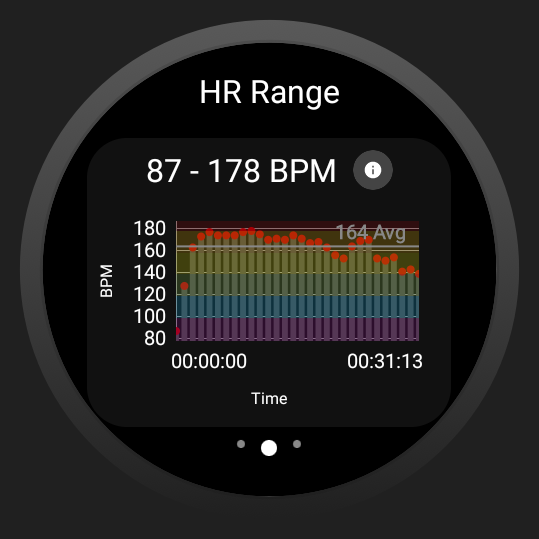
\includegraphics[width=0.5\linewidth]{dissertation//dissImages/HRRangeGraph.png}
    \caption{Enter Caption}
    \label{fig:enter-label}
\end{figure}

There are six different highlighted zones representing different levels of heart rate intensity:

\begin{itemize}
    \item \textbf{Zone 1 (Sedentary)} - This level indicates a heart rate less than 50\% of your theoretical maximum heart rate, representing a healthy resting heart rate
    \item \textbf{Zone 2 (Very Light)} - This level represents 50-60\% of your theoretical maximum heart rate, great for improving overall health and helping recovery
    \item \textbf{Zone 3 (Light)} - This level represents 60-70\% of your theoretical maximum heart rate, great for improving basic endurance and fat-burning
    \item \textbf{Zone 4 (Moderate)} - This level represents 70-80\% of your theoretical maximum heart rate, great for improving aerobic fitness
    \item \textbf{Zone 5 (Hard)} - This level represents 80-90\% of your theoretical maximum heart rate, great for increasing maximum performance
    \item \textbf{Zone 6 (Extreme)} - This level represents 90-100\% of your theoretical maximum heart rate, great for developing maximum performance and speed
\end{itemize}

These zones have a different colour scheme to the HRR zones, however maintain a similar semi-transparent approach and are again achievable through the custom renderer. There is an information icon located at the top-right of the graph that allows users to understand what each of the coloured zones represents. The zonal highlighting values are scientifically proven intensity zones, as mentioned by \cite{8025953}

\begin{figure}[h!]
    \centering
    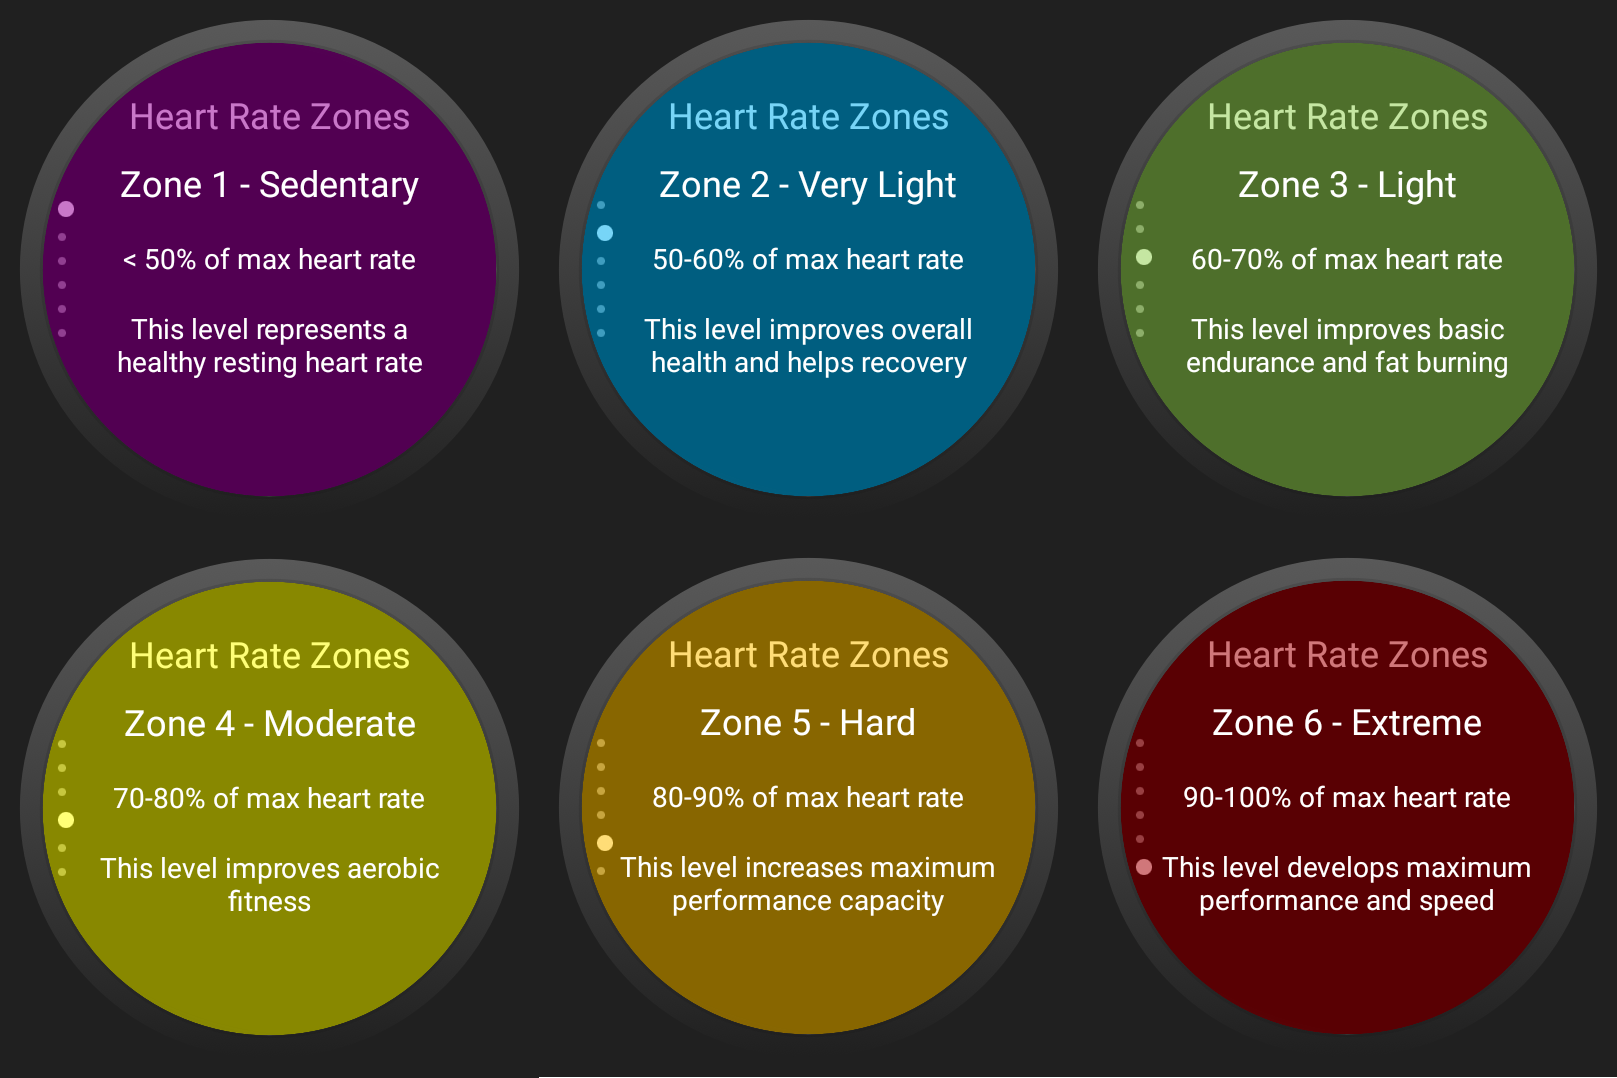
\includegraphics[width=0.75\linewidth]{dissertation//dissImages/HRZonesCombined.png}
    \caption{Enter Caption}
    \label{fig:enter-label}
\end{figure}

\subsection{HRR Comparison}
\label{sec:hrrcomparison}

To compare HRR readings previously, users would have to flick between two different readings potentially even in different workouts. It was also often difficult to compare that way due to the different heart rate values in a HRR reading changing the y-axis scale. The HRR comparison page fixes this problem, giving users a simple graph to directly compare two HRR readings from any of their workouts.

Once a user has clicked on the comparison icon, as described at the end of section \ref{sec:hrrgraph}, to compare another measurement to the one they're currently on. The user can swipe through all the HRR readings the watch has stored on the database across all their workouts, including the current one. Clicking on another reading then provides the comparison between the selected measurement and the current one through a graph shown below.

\begin{figure}[h!]
    \centering
    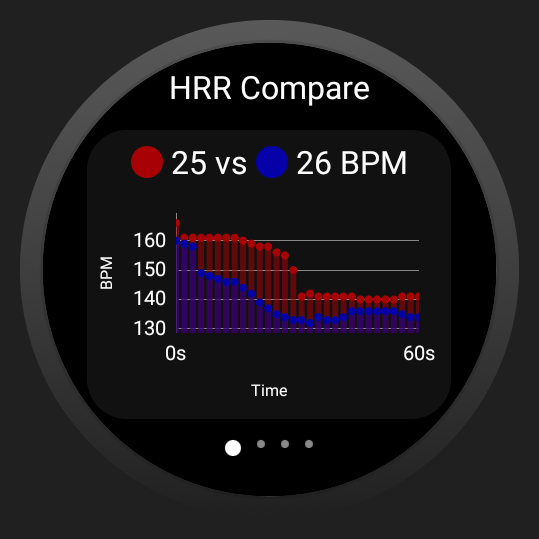
\includegraphics[width=0.5\linewidth]{dissertation//dissImages/HRRCompareGraph.png}
    \caption{Enter Caption}
    \label{fig:enter-label}
\end{figure}

The plotting of the graph is done almost identically to the HRR bar chart, except for two HRR lists. These two lists are given a separate colour scheme, one red and the other blue, to differentiate between the two plots. By plotting on the same graph, it fixes the issue of scaling while also being able to compare the heart rates across the minute-long interval. Above the graph, the two HRR values are shown, with coloured indicators as the key for the graph. Swiping across also allows users to see the two readings plotted individually if they want to look closer at one of the two measurements.

%==================================================================================================================================
\chapter{Evaluation} 
\label{sec:eval}

\section{Pilot Study}
\label{sec:pilotstudy}

\subsection{Overview}
\label{sec:pilotoverview}

The pilot study aimed to evaluate the real-world functionality and practicality of the application on a smaller scale to detect usability and functionality issues early. The study involved myself and an external evaluator analysing the application’s performance during exercise. Any issues found during the pilot study could be rectified early to ensure the broader user study was fluent. 

The pilot study was carried out in an hour-long football session. This allowed me to stress test the application, where the large number of breaks in running and more generally the amount of data being collected and processed by the application would give a thorough overview of the functionality and performance over extended periods.

Feedback from the pilot study was gathered through word-of-mouth. I asked the evaluator about their understanding of the application, questioning if there was any time they did not understand what to do or what was going on. 

\subsection{Results}
\label{sec:pilotresults}

Upon the first attempt at running the pilot study, I noticed that after approximately half an hour the watch had only tracked 5 seconds. This was a bug never previously experienced through the auto-ethnography and it was key to fix before the wider user studies. This problem was related to the WakeLock functionality within Android. When carrying out the auto-ethnography, the application was connected to my laptop for debugging and therefore the application never entered a ‘dose’ state, where the processor puts non-native apps to sleep to save resources. However, the pilot study was carried out disconnected from my laptop, meaning the application could easily be put into this ‘dose’ state. This interfered with the sensor data necessary to update the application and caused the auto-pausing functionality described in section \ref{sec:autohrr} to function incorrectly. This issue was mitigated by ensuring the application acquired an Android WakeLock when a user started a new workout, preventing the application from entering this ‘dose’ state and maintaining the application’s functionality. After the unsuccessful first attempt of running a pilot study, this issue was checked in the following week as part of my second attempt at a pilot study.

There were another two key points raised with the second iteration of pilot testing:

\begin{itemize}
    \item The time tracked on the smartwatch felt inaccurate compared to how long exercising for, with one hour of football equating to 25 minutes of activity according to the watch
    \item The evaluator also reported the watch “gave some weird vibrations” and he “couldn’t understand the meaning of these vibrations”
\end{itemize}

This prompted another two fixes for the application before the user studies. 

Firstly, the accuracy for detecting movement was adequately accurate when running at a fair pace, however was too strict when running at lighter paces. To address this, I reduced the hyperparameter determining the amount of movement required to class as being stopped, as well as increasing the time window it averages the movement across from 2 seconds to 3 seconds. This overall caused a slight but significant decrease in the sensitivity to users taking breaks and had a much more desired effect from the algorithm at slower speeds.

It was clear to see how the vibrations could be confusing to a user not aware of how the background system works, and it was an oversight to assume users would understand what a vibration indicated. To address this, I implemented an overlay that would trigger if some movement was detected. Whenever the toggle for changing the isPaused state - mentioned in section \ref{sec:autohrr} - it would also trigger the launch of this overlay, telling the user they had either paused or continued their workout. This overlay could then work alongside the vibrations already providing feedback to the user.

Once these final issues were rectified, I was ready to plan and carry out the wider user study to gather more feedback.

\section{User Studies}
\label{sec:userstudies}

\subsection{Aims}
\label{sec:userstudyaims}

The user study aimed to assess several components of the application, presenting evidence for future work and design changes to be made. The main aim of the application as stated in section \ref{aims} is to provide a way for users to intuitively track their heart rate recovery. This is quite a large area to assess, so has been broken down into three smaller components to help answer the main question:

\begin{enumerate}
    \item Evaluating the intuitiveness of the design of the application. For some of my evaluators, this was their first time using a smartwatch. It should be the case that they can use the application relatively intuitively based on similar applications on other mobile devices. This includes the design of the application and graphs but also the navigation and interaction for the users
    \item Evaluating the clarity of certain features and functionality designed to boost the user's understanding of their HRR and heart health. One of the main issues identified with the Apple Watch’s approach to HRR was how hidden the feature was for users to find, as noted in section \ref{sec:applewatch}. It was important to try and design the application to avoid falling into the same trap
    \item Evaluating the usefulness and practicality of the application. While this application was only initially designed with running in mind, it would be useful to see how it performs when put under a variety of different workouts and exercises. Part of my future work will look at assessing this performance to expand the available workouts, as well as fixing any features people felt were missing from the application.
\end{enumerate}

\subsection{Experiment Design}
\label{sec:userstudydesign}

The experiment involved users taking a Mobvoi TicWatch Pro 3 with the application pre-installed and in a “fresh install” state, meaning the application appeared as it would for its first download. This gave users the full experience of setting up the application for themselves. Users were assigned two separate tasks to complete while tracking a workout with the watch application:

\begin{enumerate}
    \item Completing a 10-minute run with a 2-minute break 5 minutes in, meaning they would run for five minutes, stop for two, then run for another five.
    \item Another unspecified exercise for any length of period, to assess the performance of other workout types
\end{enumerate}
Following the completion of these two exercises, users were then tasked with completing a survey that covered three main areas:

\begin{itemize}
    \item Intuitive Design questions - Assessing the intuitiveness of the design and navigation throughout the application
    \item Task-based questions - Assessing the user’s ability to interpret results and find knowledge-boosting features
    \item Application Practicality questions - Assessing the usefulness of the application and the performance of the application on the other exercise carried out by the us
\end{itemize}

Each of these areas would provide valuable insight into our aims outlined in section \ref{aims}

\subsection{Results}
\label{sec:userstudyresults}

A total of 7 participants were gathered from a convenience sample, all of which completed all aspects of the evaluation. 6 participants fell under the age range of 18-24 years, with the remaining falling under the 25-34 range. All 7 participants identify as male. Most of the participants have a strong technical background with 6 studying a computing-related degree, with the remaining having no background in computing.

Quantitative questions were evaluated against the Likert scale, with 1 being a strongly negative response and 5 being a strongly positive response. Each question had the scale labelled more specifically to ensure a clear understanding of the scale for the respondent.

\noindent\mbox{}\\
\subsubsection{Intuitive Design Questions}
\noindent\mbox{}\\

When asked about the navigational process throughout the application, participants found the process very intuitive. Regarding the question “How easy do you find the application to navigate?”, all participants answered above a rating of 4, with one participant reviewing it a 5. Users also found the application to be consistent with similar mobile applications, with an average rating of 4 across all participants (standard deviation = 0.40)

\begin{figure}[h!]
    \centering
    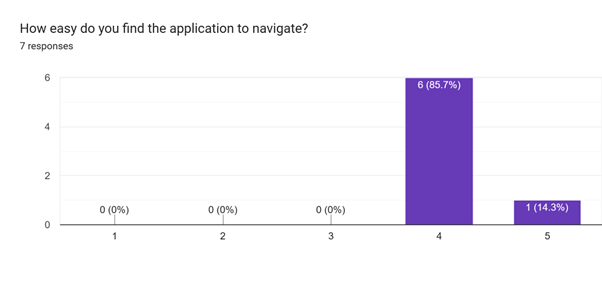
\includegraphics[width=0.75\linewidth]{dissertation//dissImages/NavigationEasy.png}
    \caption{Enter Caption}
    \label{fig:enter-label}
\end{figure}

\begin{figure}[h!]
    \centering
    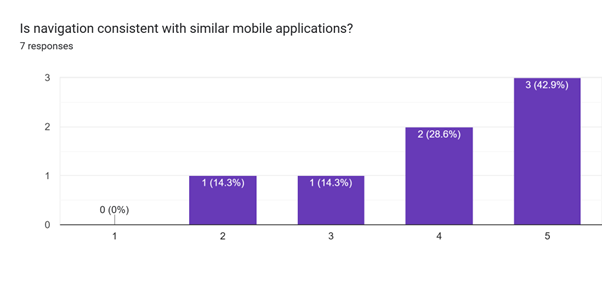
\includegraphics[width=0.75\linewidth]{dissertation//dissImages/NavigationConsistency.png}
    \caption{Enter Caption}
    \label{fig:enter-label}
\end{figure}

Another key aim of the study was to assess the design and clarity of the graphs presented at the end of a workout. Evaluators reported an average score of 3.86 when considering how easy the post-workout graphs (HRR and HR range) were to understand (standard deviation = 0.99). The respondents also reviewed the clarity of the graph colours at a very high average rating of 4.43 (standard deviation = 0.73).

\begin{figure}[h!]
    \centering
    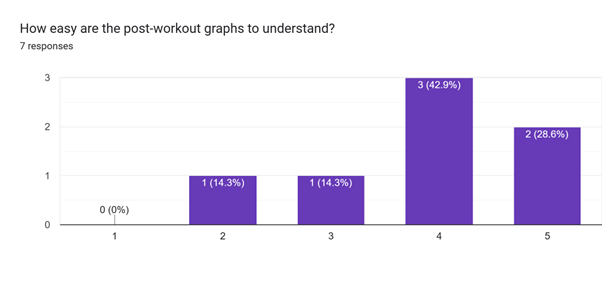
\includegraphics[width=0.75\linewidth]{dissertation//dissImages/GraphEasy.png}
    \caption{Enter Caption}
    \label{fig:enter-label}
\end{figure}

\begin{figure}[h!]
    \centering
    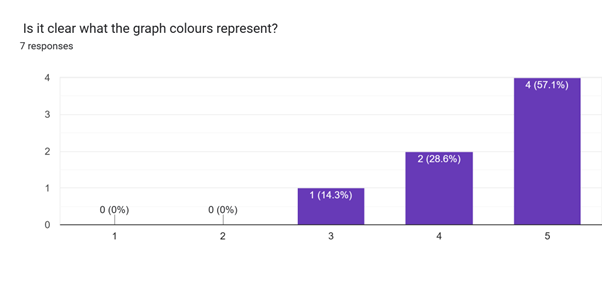
\includegraphics[width=0.75\linewidth]{dissertation//dissImages/GraphColour.png}
    \caption{Enter Caption}
    \label{fig:enter-label}
\end{figure}

Participant’s opinions on the vibrations given by the system when toggling between a ‘paused’ and ‘resumed’ state were very mixed however generally the vibrations were not appreciated with an average rating of just 2.86 (standard deviation = 1.25).

\begin{figure}[h!]
    \centering
    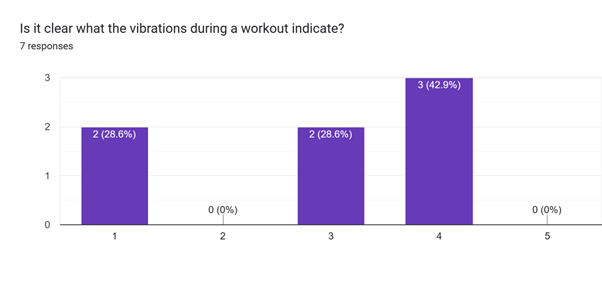
\includegraphics[width=0.75\linewidth]{dissertation//dissImages/Vibrations.png}
    \caption{Enter Caption}
    \label{fig:enter-label}
\end{figure}


\noindent\mbox{}\\
\subsubsection{Post-Exercise Task-Based Questions}
\noindent\mbox{}\\

Based on the responses to the task-based questions, I could gather whether or not the user had correctly completed or interpreted what the task required. The tasks set to complete were as follows:

\begin{itemize}
    \item \textbf{Task 1} required users to state their average heart rate during their running exercise. This is shown as a grey line with a value, as explained in section \ref{sec:hrrangegraph}.
    \item \textbf{Task 2} asked users to state the intensity zone this average heart rate fell under.
    \item \textbf{Task 3} asked users what percentage band of their theoretical maximum heart rate this fell under.
    \item \textbf{Task 4} asked users what their different HRR measurements were, ensuring they knew that the application stored multiple HRR readings for a workout
    \item \textbf{Task 5} asked users to complete a comparison of two different HRR readings, prompting them to navigate to the HRR compare feature described in section \ref{sec:hrrcomparison}
    \item \textbf{Task 6} asked users what their active running time and total exercise duration was throughout the run
\end{itemize}

\begin{table}[h!]
    \centering
    \caption{Enter Caption} % MENTION ASTERISK MEANINGS
    \label{fig:enter-label}
    \begin{tabular}{|l|ccccccc|r|}
        \hline  
        Participant no. & 1 & 2 & 3 & 4 & 5 & 6 & 7 & Task Completion \\
        \hline
        Task 1 & \cmark & \cmark & \cmark & \xmark & ?* & \cmark & \cmark & 5/6 (83.3\%)\\
        Task 2 & \cmark & \cmark & \cmark & \cmark & ?* & \cmark & \cmark & 6/6 (100\%)\\
        Task 3 & \cmark & \cmark & \cmark & \cmark & ?* & \cmark & \xmark & 6/6 (100\%)\\
        Task 4 & \xmark & \cmark & \xmark & \xmark & \cmark & \cmark & \xmark & 3/7 (42.9\%)\\
        Task 5 & \xmark & \cmark & \xmark & \xmark & \cmark & \cmark & \xmark & 3/7 (42.9\%)\\
        Task 6 & \cmark & \cmark & \cmark & \cmark & \cmark & \cmark & \cmark** & 7/7 (100\%)\\
        \hline
    \end{tabular}
\end{table}

\noindent\mbox{}\\
\subsubsection{Application Practicality}
\noindent\mbox{}\\

The overall concept of the application received high praise from evaluators, with an average review of 4.71 (standard deviation = 0.45). This goes hand in hand with how important participants found their heart health information while working out, with an average review of 4.0 (standard deviation = 1.41)

\begin{figure}[h!]
    \centering
    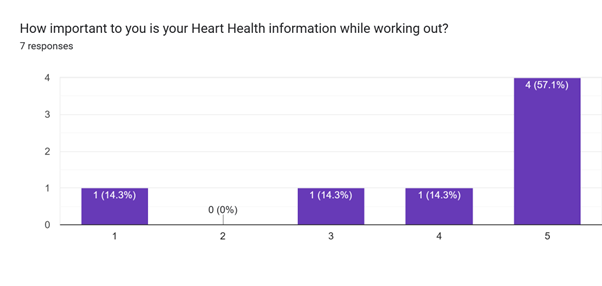
\includegraphics[width=0.75\linewidth]{dissertation//dissImages/HeartImportant.png}
    \caption{Enter Caption}
    \label{fig:enter-label}
\end{figure}

\begin{figure}[h!]
    \centering
    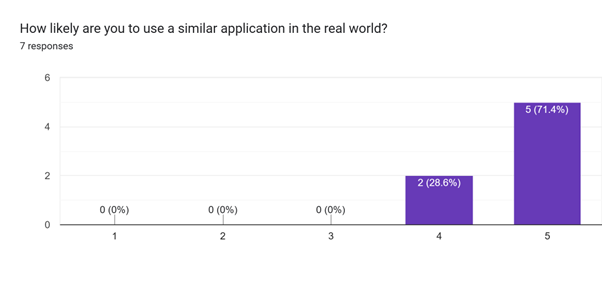
\includegraphics[width=0.75\linewidth]{dissertation//dissImages/UseApplication.png}
    \caption{Enter Caption}
    \label{fig:enter-label}
\end{figure}


The auto-pausing functionality proved divisive for participants, with the highest variance in results across all the quantitative questions asked. The average review of the effectiveness was 2.86 with a huge standard deviation of 1.46

\begin{figure}[h!]
    \centering
    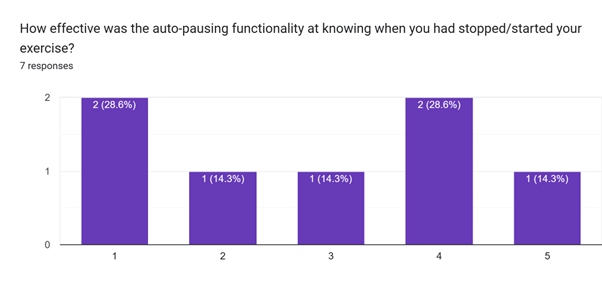
\includegraphics[width=0.75\linewidth]{dissertation//dissImages/PauseEffective.png}
    \caption{Enter Caption}
    \label{fig:enter-label}
\end{figure}

\subsection{Analysis and Discussion}
\label{sec:userstudyanalysis}

\noindent\mbox{}\\
\subsubsection{Intuitive Design}
\noindent\mbox{}\\

One of the main aims of the application is to allow for easy accessibility to HRR. The results show that the navigational design of the application was overall very positive (ENTER FIGURE REFERENCE HERE). Some evaluators did report that they were “unsure at first with navigation”, however found it “very intuitive and easy to use” after some adjusting to the new system. Participant 6 explained how “the little dots showed whereabouts I was so I never got lost”, showing that while this navigational technique may have been new for some users, the design choices I made to assist with navigational context proved very effective in directing users.

The graphical representation of the HRR and heart rate range was also very well received as evident from (ENTER FIGURE REFERENCE HERE), with four participants expressing how they liked the “clear and basic” and “easy to understand” design. Participant 7 did note that they “weren’t quite sure what they were representing”. This feedback indicates that while the application may logically represent HRR, it needs to have a clearer explanation of what it is measuring and displaying to the user.

Giving users multimodal context of the state of the application was a feature designed to let users know when the application paused state had toggled without needing to visually check if it had toggled. This was implemented in the form of vibrations, however the system received mixed feedback with the question receiving the second-highest standard deviation across the whole evaluation at 1.25. The overall negative feedback of the feature means it will need a redesigned implementation and further evaluation to ensure the desired effect. This is discussed further in section \ref{sec:futurework}.

\noindent\mbox{}\\
\subsubsection{Post-Experiment Task-Based Questions}
\noindent\mbox{}\\

The task-based questions provided valuable insight into how accessible and intuitive the features implemented were. Notably, Participant 5 and Participant 7 raised issues found with the functionality of the application itself. 

Participant 5 raised a bug where the Heart Rate Range graph described in section \ref{sec:hrrangegraph} did not render, instead displaying the message “Not Enough Data”. This bug however, did not prevent the HRR graph from displaying as normal and was unique only to their running workout as opposed to their other exercise. 

Participant 7 experienced an issue with the Active Timer functionality, where the timer remained at ‘00:00:00’ throughout the workout. This could be an issue relating to the accelerometer, as I had issues with the heart rate monitor where it would consistently return the value “-2” and not the user’s actual heart rate. This issue was temporarily solved by showing a “Sensor Error” message to the user and instructing in the experiment outline for users to remove and replace the watch on the wrist and restart the exercise. A more permanent fix to this issue would be validation of the sensor readings, where incorrect or impossible readings could trigger the application to unregister and re-register the sensor listener to restart the sensor.

Most tasks achieved a high success rate, with task one achieving over 80\% completion rate while tasks two, three and six all saw a 100\% success rate in task completion. This emphasises the graph implementation was overall very clear for participants to understand. The active and total time was also very intuitive to find and understand for the user.

Both tasks 4 and 5 only saw a 42.9\% success rate, with only 3 of the 7 participants finding these features. 

\begin{itemize}
    \item Task 4 challenged users to realise the vertical swiping to find more HRR readings. The application aimed to use page indicators, similar to what was used for horizontal pagination, however this was not clear enough to most users. To improve this feature, the application could help users navigate more directly, with a downwards arrow on the screen to indicate to users there is more info vertically as well as horizontally.
    \item Task 5 challenged users to find the compare functionality within the HRR graph. This was achieved poorly, due to the button being too small and unclear as to what its function was. The information button is intuitive as the ‘information’ symbol is known universally, however the ‘compare’ icon is not as intuitive. This could be fixed by finding some other way of navigating to the comparison page, perhaps swiping left on a HRR reading to compare.
\end{itemize}

\noindent\mbox{}\\
\subsubsection{Application Practicality}
\noindent\mbox{}\\

People are keen to keep track of their heart health with all participants scoring a 4 or above on how likely they are to use the application. The desire to use my application is evidence of the gap in current applications and is a strong indication of a successful project.

Considering the application’s performance on other exercises, the variety of other exercises can be categorised into three different types:

\begin{itemize}
    \item \textbf{Consistent Arm Movement} - Activities where the user’s arm is constantly moving at a relatively fast pace, including rowing and running (with natural duration and breaks)
    \item \textbf{Intermittent Arm Movement} - Activities that see large fluctuations between fast and slow movement, such as badminton and football
    \item \textbf{Negligible Arm Movement} - Activities where there is rarely any fast arm movement, such as weightlifting, a ‘leg workout’ and scrambling
\end{itemize}

From qualitative feedback, the feedback on the application’s performance follows what was theorised. 

The application performs “functionally the same” when considering an exercise with lots of arm movement, with Participant 7 stating their rowing exercise showed statistics “similar to the machine”. 

With exercises less consistent with arm movement the application was still functional for HRR readings, with the data being “more clear because of [the] longer time” according to Participant 2. However, the functionality of the workout pausing mechanism did perform questionably, with Participant 2 stating they “played football for 1 hour” and the app only reported “10 minutes active time”. This is further supported by Participant 5 stating “The application was pausing my workout all the time, and vibrations were disrupting my workout”. As discussed earlier, the vibration system will need to be redesigned in future to make it more user-friendly.

Finally, negligible arm movement exercises performed overall poorly as anticipated. Participant 3 appreciated “it performed well when running” but stated, “When it came to weightlifting it was surprisingly poor”. This emphasises that workouts with less overall arm movement would require a different way of triggering HRR readings and in general, differentiating between users taking a break and actively moving. Similar to above, the pausing functionality would need to be reassessed for this use case and is something discussed further in \ref{sec:futurework}

\noindent\mbox{}\\
\subsubsection{General Discussion}
\noindent\mbox{}\\

After completing the evaluation, I asked the participants some questions about how everything went and if they experienced any issues. Participant 4 explained that they removed the watch accidentally before remembering they had not ended the workout. This resulted in their heart rate graph being skewed. This is an oversight of the application that could be solved by simply not storing values of 0 or below, allowing for the heart rate graph to remain accurate.

More general feedback received from Participants 2 and 3 is that the idea of an “Active Timer” and “Total Duration” is confusing. They stated that they felt when the watch entered a paused state, that it was no longer tracking their workout. This is inaccurate, everything is still being tracked with the only impact being the “Active Timer” is paused, however the design of the pausing effect gives the impression that more is happening.

%==================================================================================================================================
\chapter{Conclusion}   
\label{sec:conclusion}

\section{Future Work}
\label{sec:futurework}

From the evaluation of the application, there are several features desired for the future development of the project. 

The vibration effects of the application were reviewed negatively, highlighting a key area for change. The desired effect of the vibration was to give users context of when the application had detected users taking a break, however the key area of annoyance was the inability to check the active workout without resulting in the app thinking the user was taking a break. While the accuracy of detecting a stop is important to accurately measure the minute-long period of doing an automatic HRR measurement, the vibration effect could be altered slightly to happen after an extended delay to not go off when the movement is stopped temporarily to check the application. 

The application could also provide more context to the user on their current heart health information during a workout. With the current design, users can view their current heart rate and their peak heart rate during a workout. This could be improved with the addition of thematic styling representing the user’s current heart rate zone, giving users more information on the intensity of their workout at a glance. Additionally, some indication of how many heart rate recovery measurements have been taken could provide the user more context about their workout, helping them decide if they have gathered enough data to review or if they want to push for more.

Moving onto larger-scale features, another development requested through the user study is an automatically starting workout. This could be a more complex issue to tackle, as it would require constantly running the application in the background to detect certain patterns in the user’s movement that could trigger an exercise starting. However, it would be another step towards automating the process of HRR measuring, therefore would pose an interesting challenge but undeniably useful feature for the future.

The application had mixed performance when tested against exercises other than running. It is likely users who will be interested in heart health information will partake in a wide variety of exercises, with this being received as feedback through the evaluation. The application should perform as expected for as many exercises as possible to accommodate users' needs. This will involve finding some other form of detecting when a user stops for a break to trigger an automatic HRR reading. The application could also allow for manual triggering of a HRR reading, counteracting the issue of HRR measuring when a user’s wrist is not moving.

Additionally, the application could collaborate with a mobile application. This mobile application could provide a platform for several new possible features, including a social media aspect where you can keep track of your friends’ performance, or introduce a challenges interface where users can sign up for challenges to aim for. In general, a mobile application will also allow for more interactivity and detail in the interface due to the bigger screen size, allowing for improved visualisations.

\section{Summary}
\label{sec:summary}

Workout and fitness trackers are becoming increasingly common with an increase in easily accessible wearable devices. However, while many of these devices and applications have access to a heart rate monitor, it is common to overlook reporting important heart health metrics like heart rate recovery.

In order to bridge this gap, I designed and developed an application that puts heart health metrics at the forefront of functionality. The application provided users with useful insight into their heart health, displaying graphs of their results for easy interpretation.

The application design was carefully considered, from the visuals of the user interface to the interaction and navigation design, in order to ensure users could navigate the application and find the information they were looking for as intuitively as possible.

The application was developed and evaluated using the Mobvoi TicWatch Pro 3. The evaluation consisted of two main stages:

\begin{itemize}
    \item \textbf{Pilot Study} - for a smaller scale high-level evaluation of the application’s functionality
    \item \textbf{User Studies} - for a more specific larger-scale evaluation of the application’s intuitiveness and practicality
\end{itemize}

The user studies aimed to raise any issues with the design of the application, as well as any features that were not understood by the user and the application’s overall practicality in the real world.

From the results, it became clear that the gap in the market was bridged by this application and users were keen to learn more about their heart health during exercise. The graphs were well received and understood by most users, allowing for a clear understanding of their HRR and what it meant for their heart health. On the flip side, the multimodular vibration effect played when toggling the paused state was not very well received, and would require future work in order to be as effective as initially desired.

The application has many potential routes for future development, including a range of smaller-scale design changes such as rethinking the vibrations and giving users context of their heart health and workout intensity during a workout.

Larger-scale developments include adding more variety of supported workouts to categorise for the user, as well as automatically starting these workouts where users may forget. The application could also collaborate with a mobile application via a web server to allow for features suited to a larger display, such as an integrated social media platform and increased result interactivity to enhance understanding of measurements taken.

%==================================================================================================================================
%
% 
%==================================================================================================================================
%  APPENDICES  

\begin{appendices}

\chapter{Appendices}
\label{sec:appendices}

\begin{figure}[h!]
    \centering
    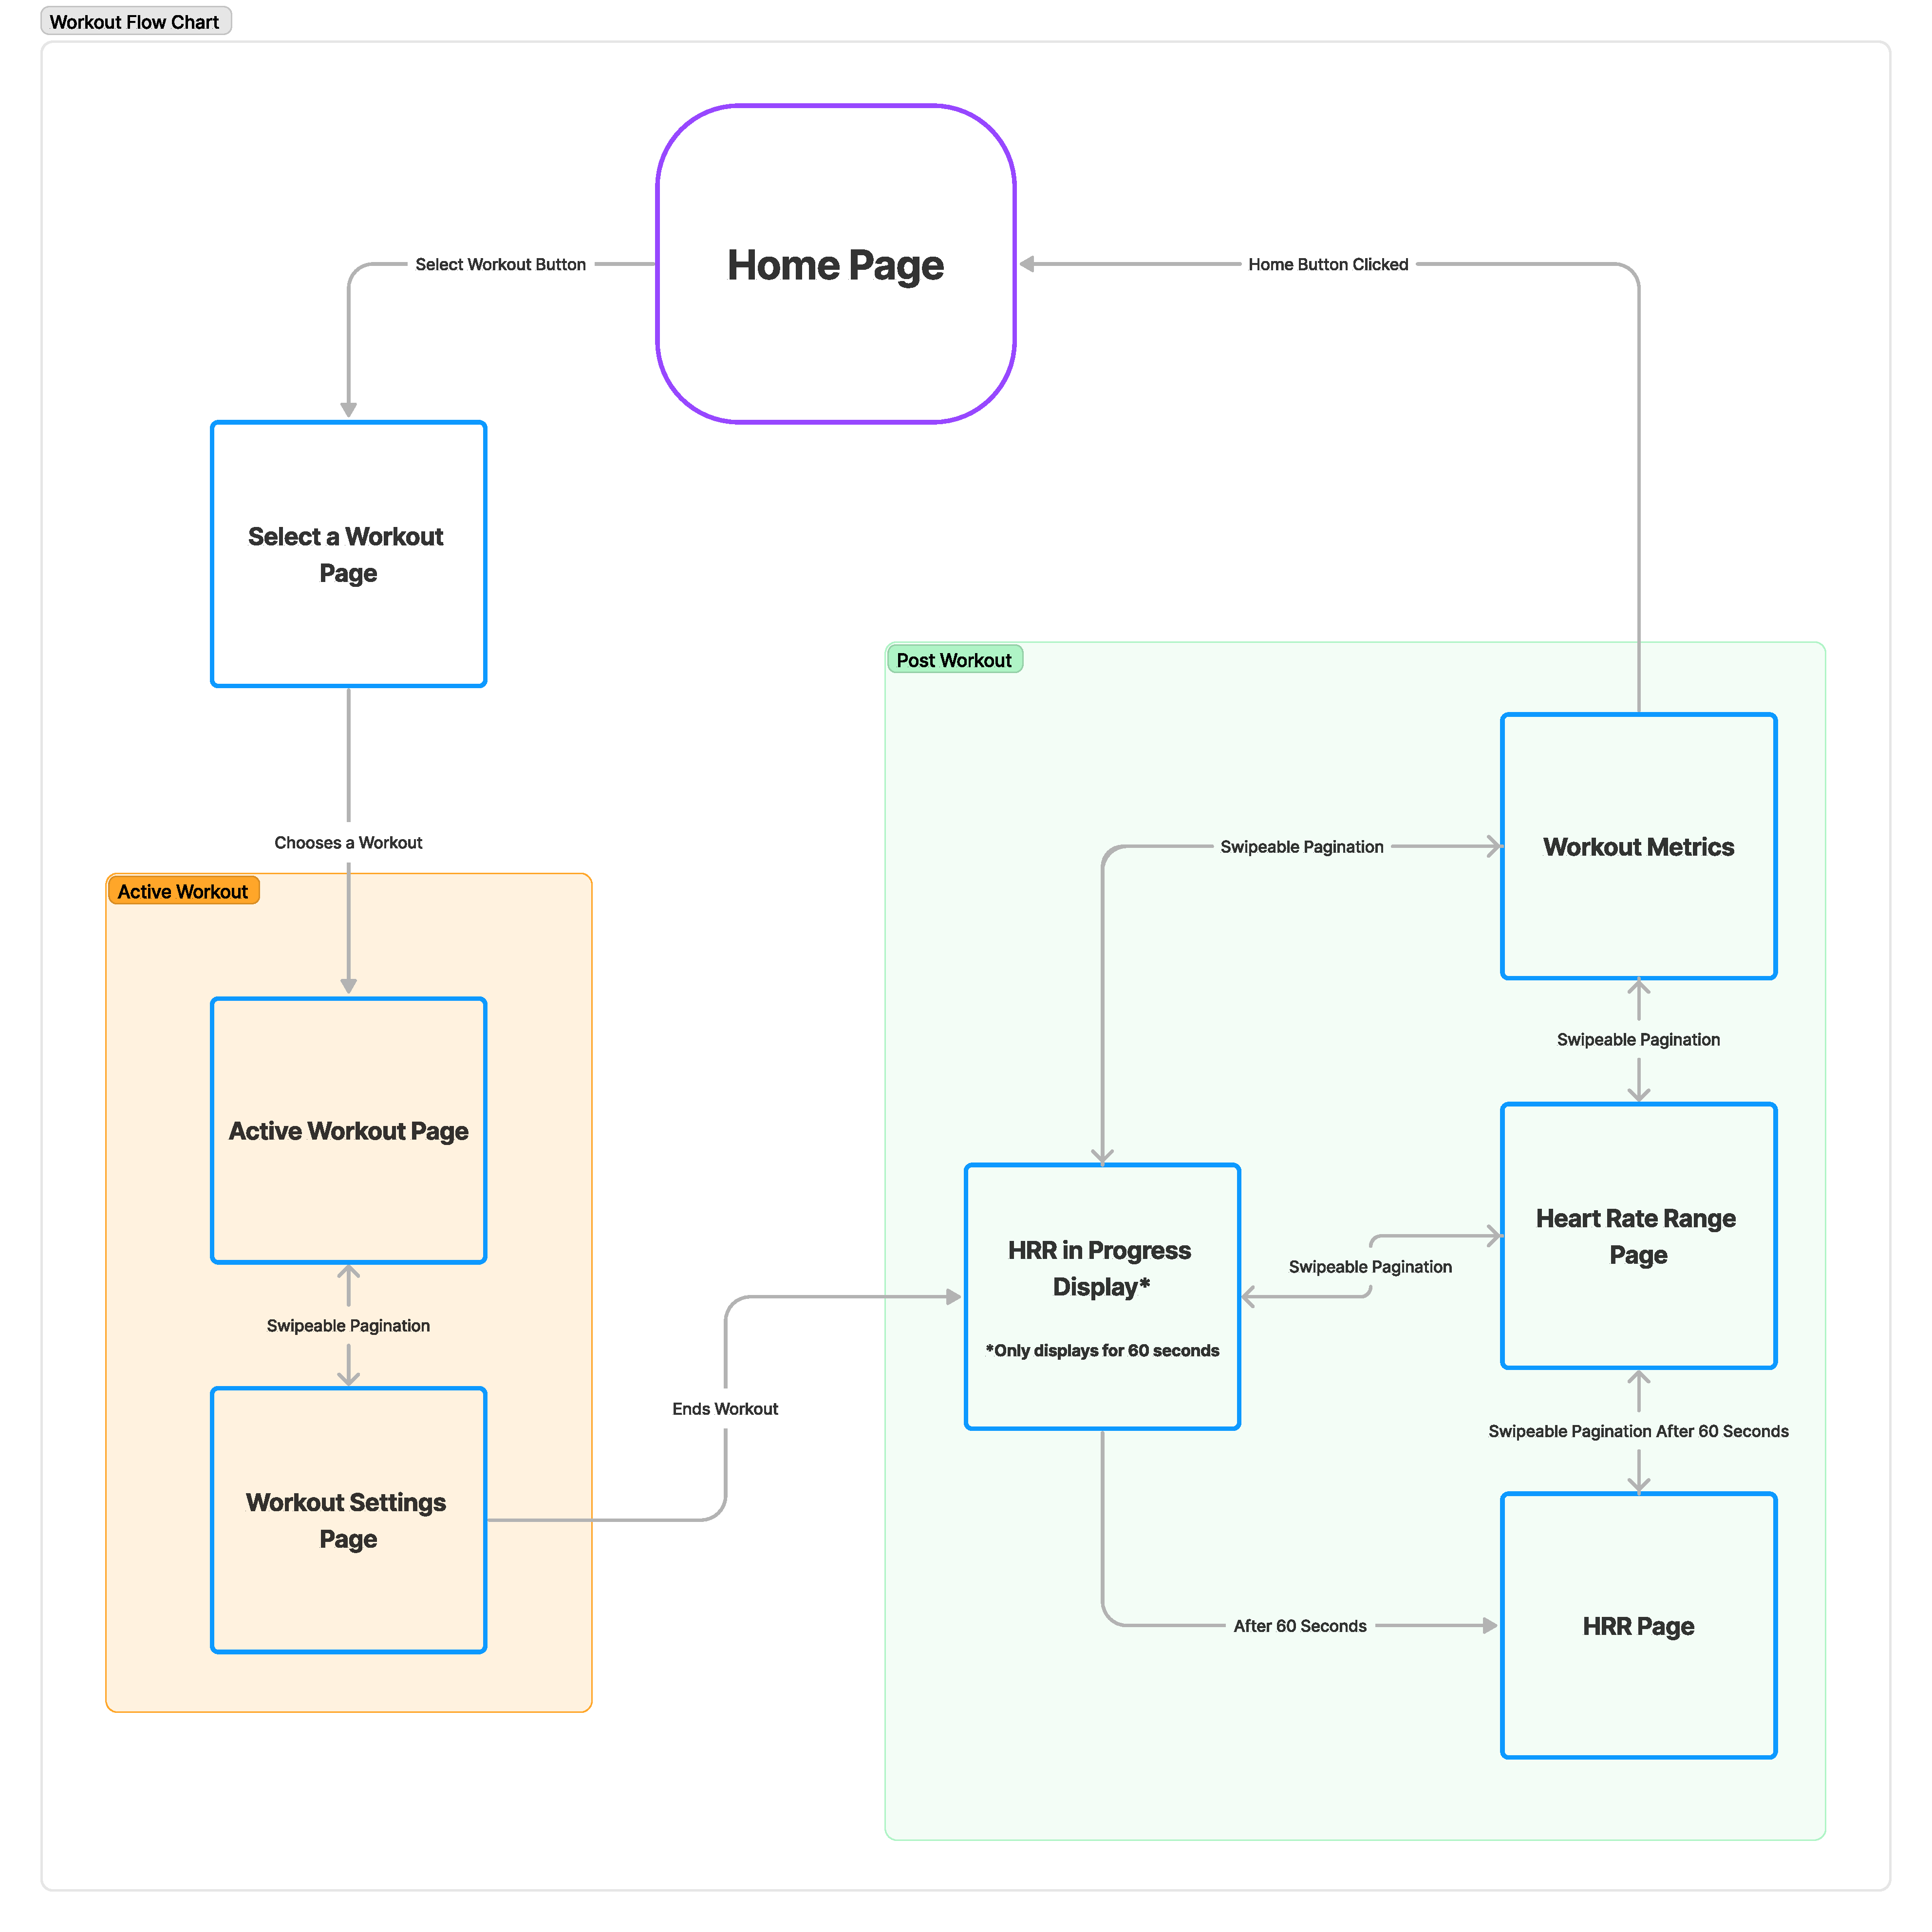
\includegraphics[width=0.75\linewidth]{dissertation//dissImages/WorkoutFlow.pdf}
    \caption{Enter Caption}
    \label{fig:enter-label}
\end{figure}

\begin{figure}[h!]
    \centering
    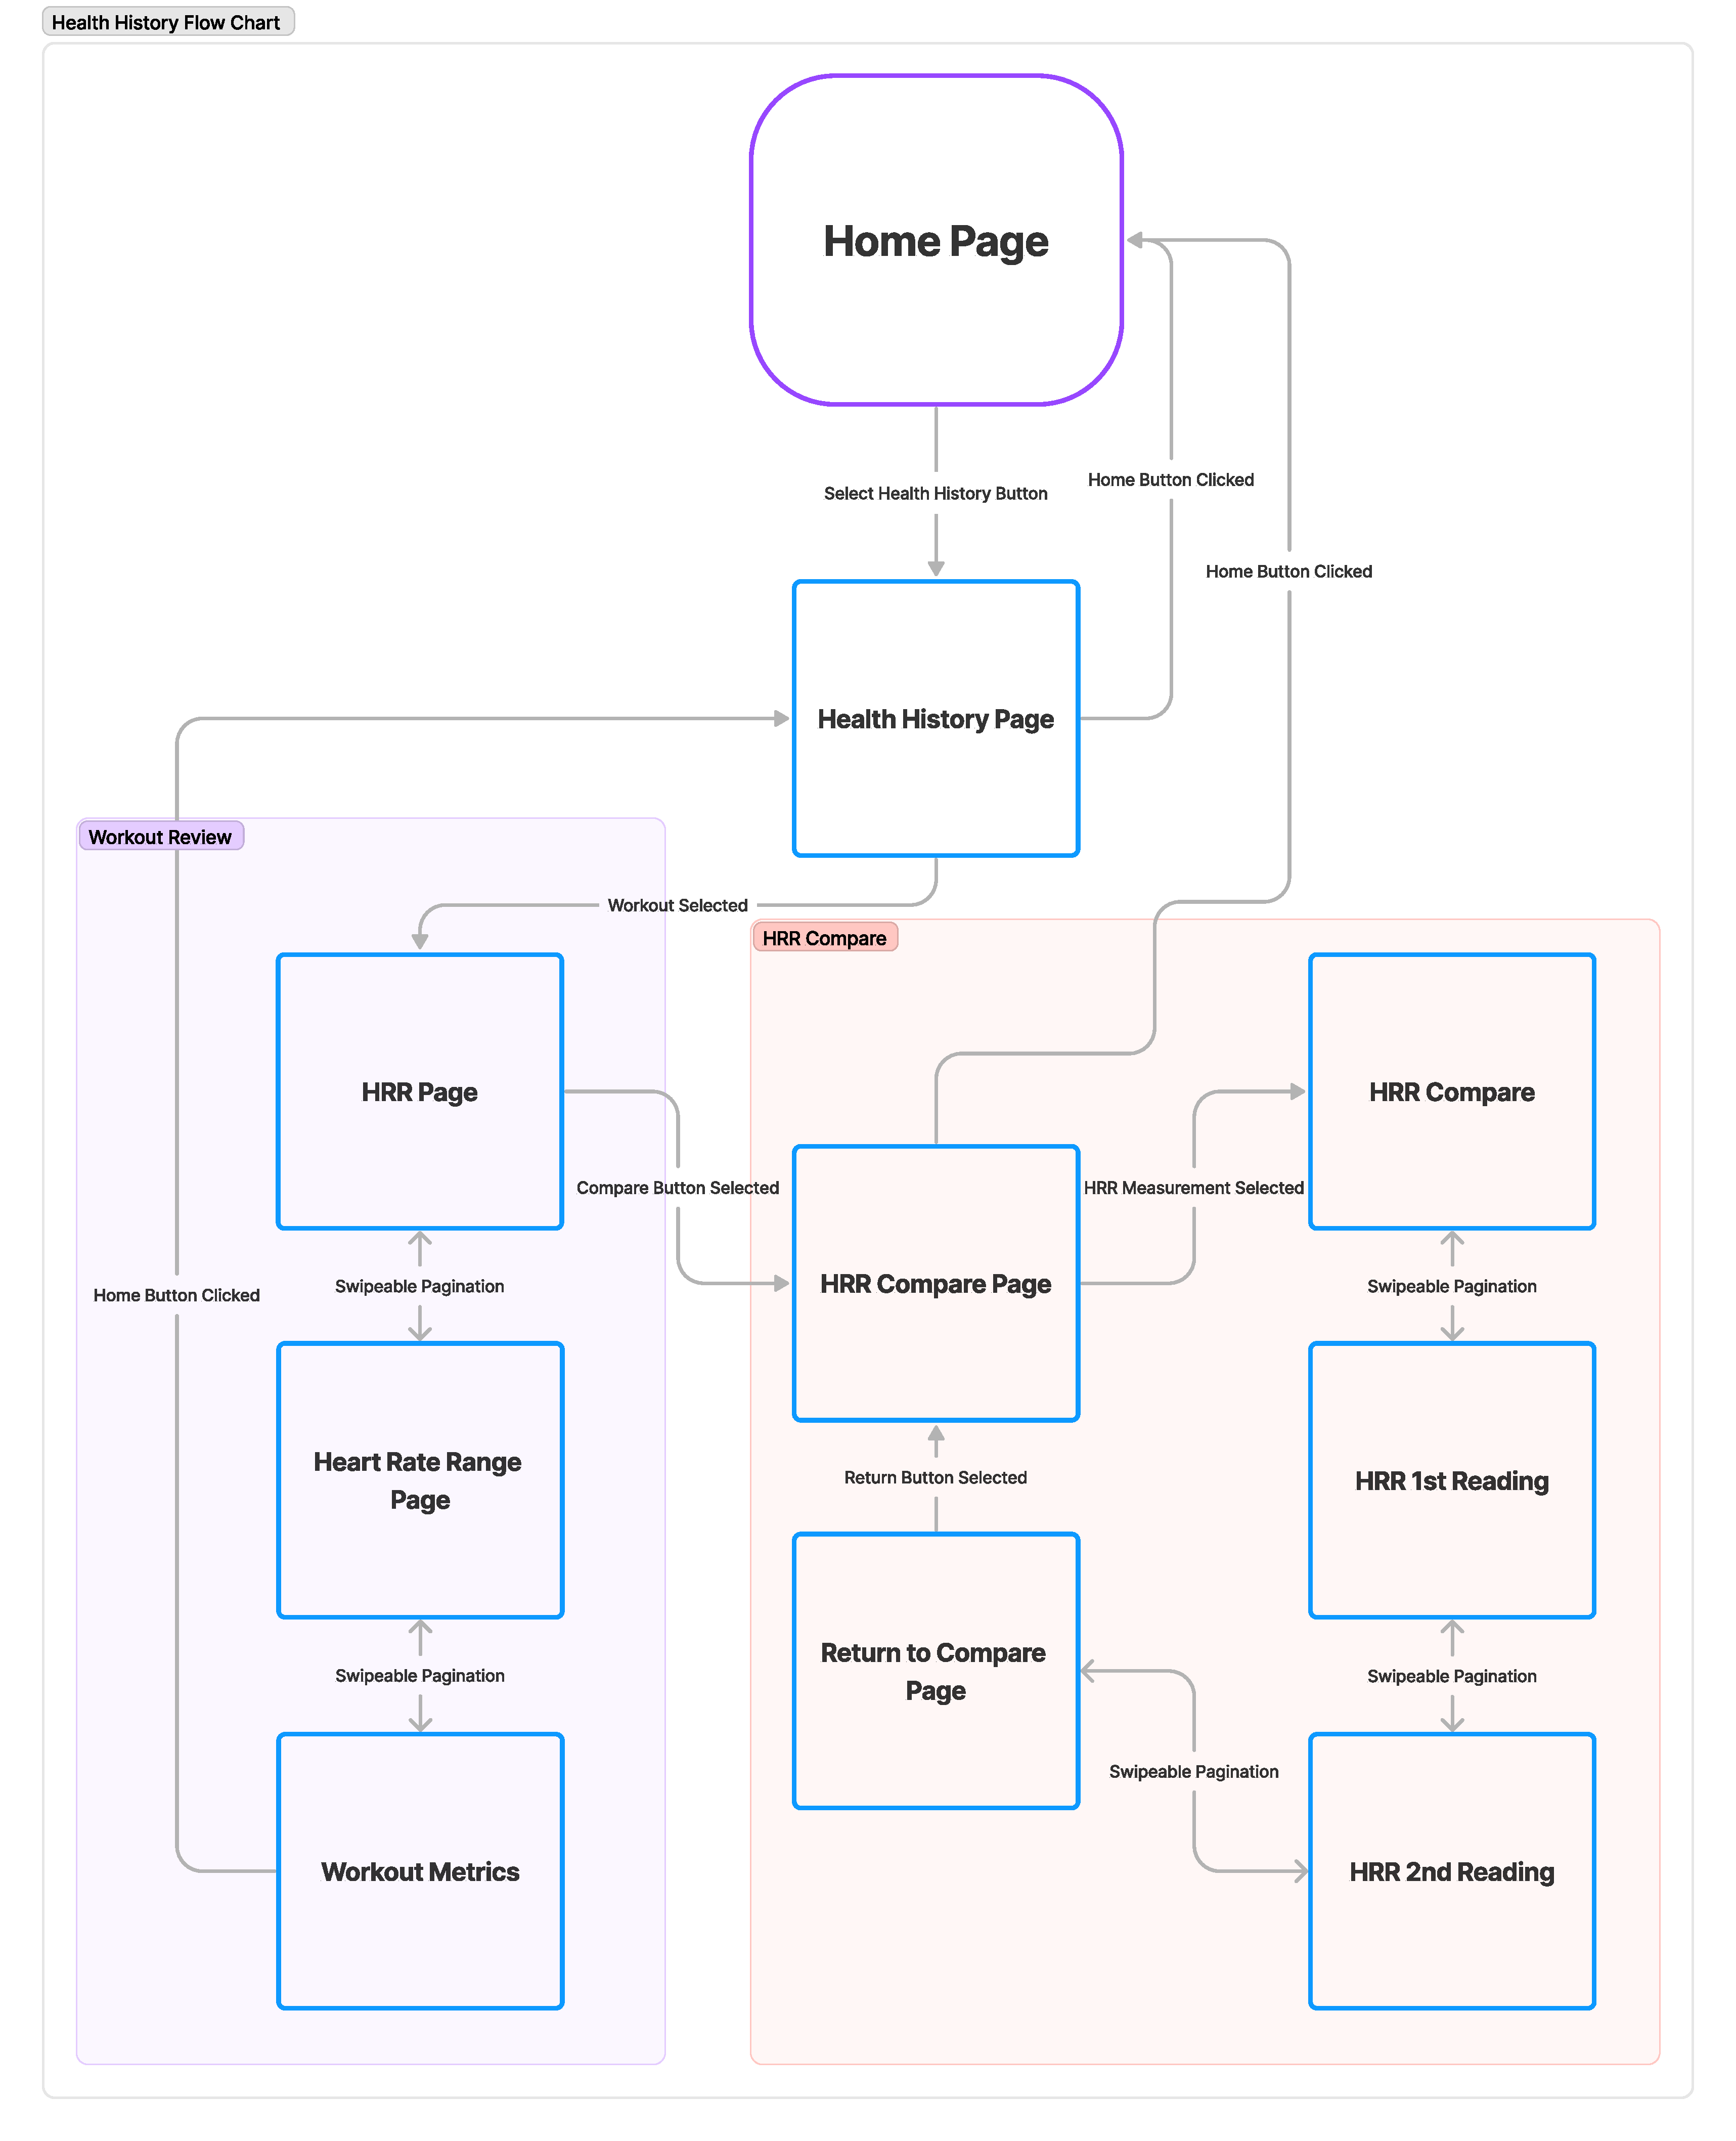
\includegraphics[width=0.75\linewidth]{dissertation//dissImages/HealthHistoryFlow.pdf}
    \caption{Enter Caption}
    \label{fig:enter-label}
\end{figure}

\begin{figure}[h!]
    \centering
    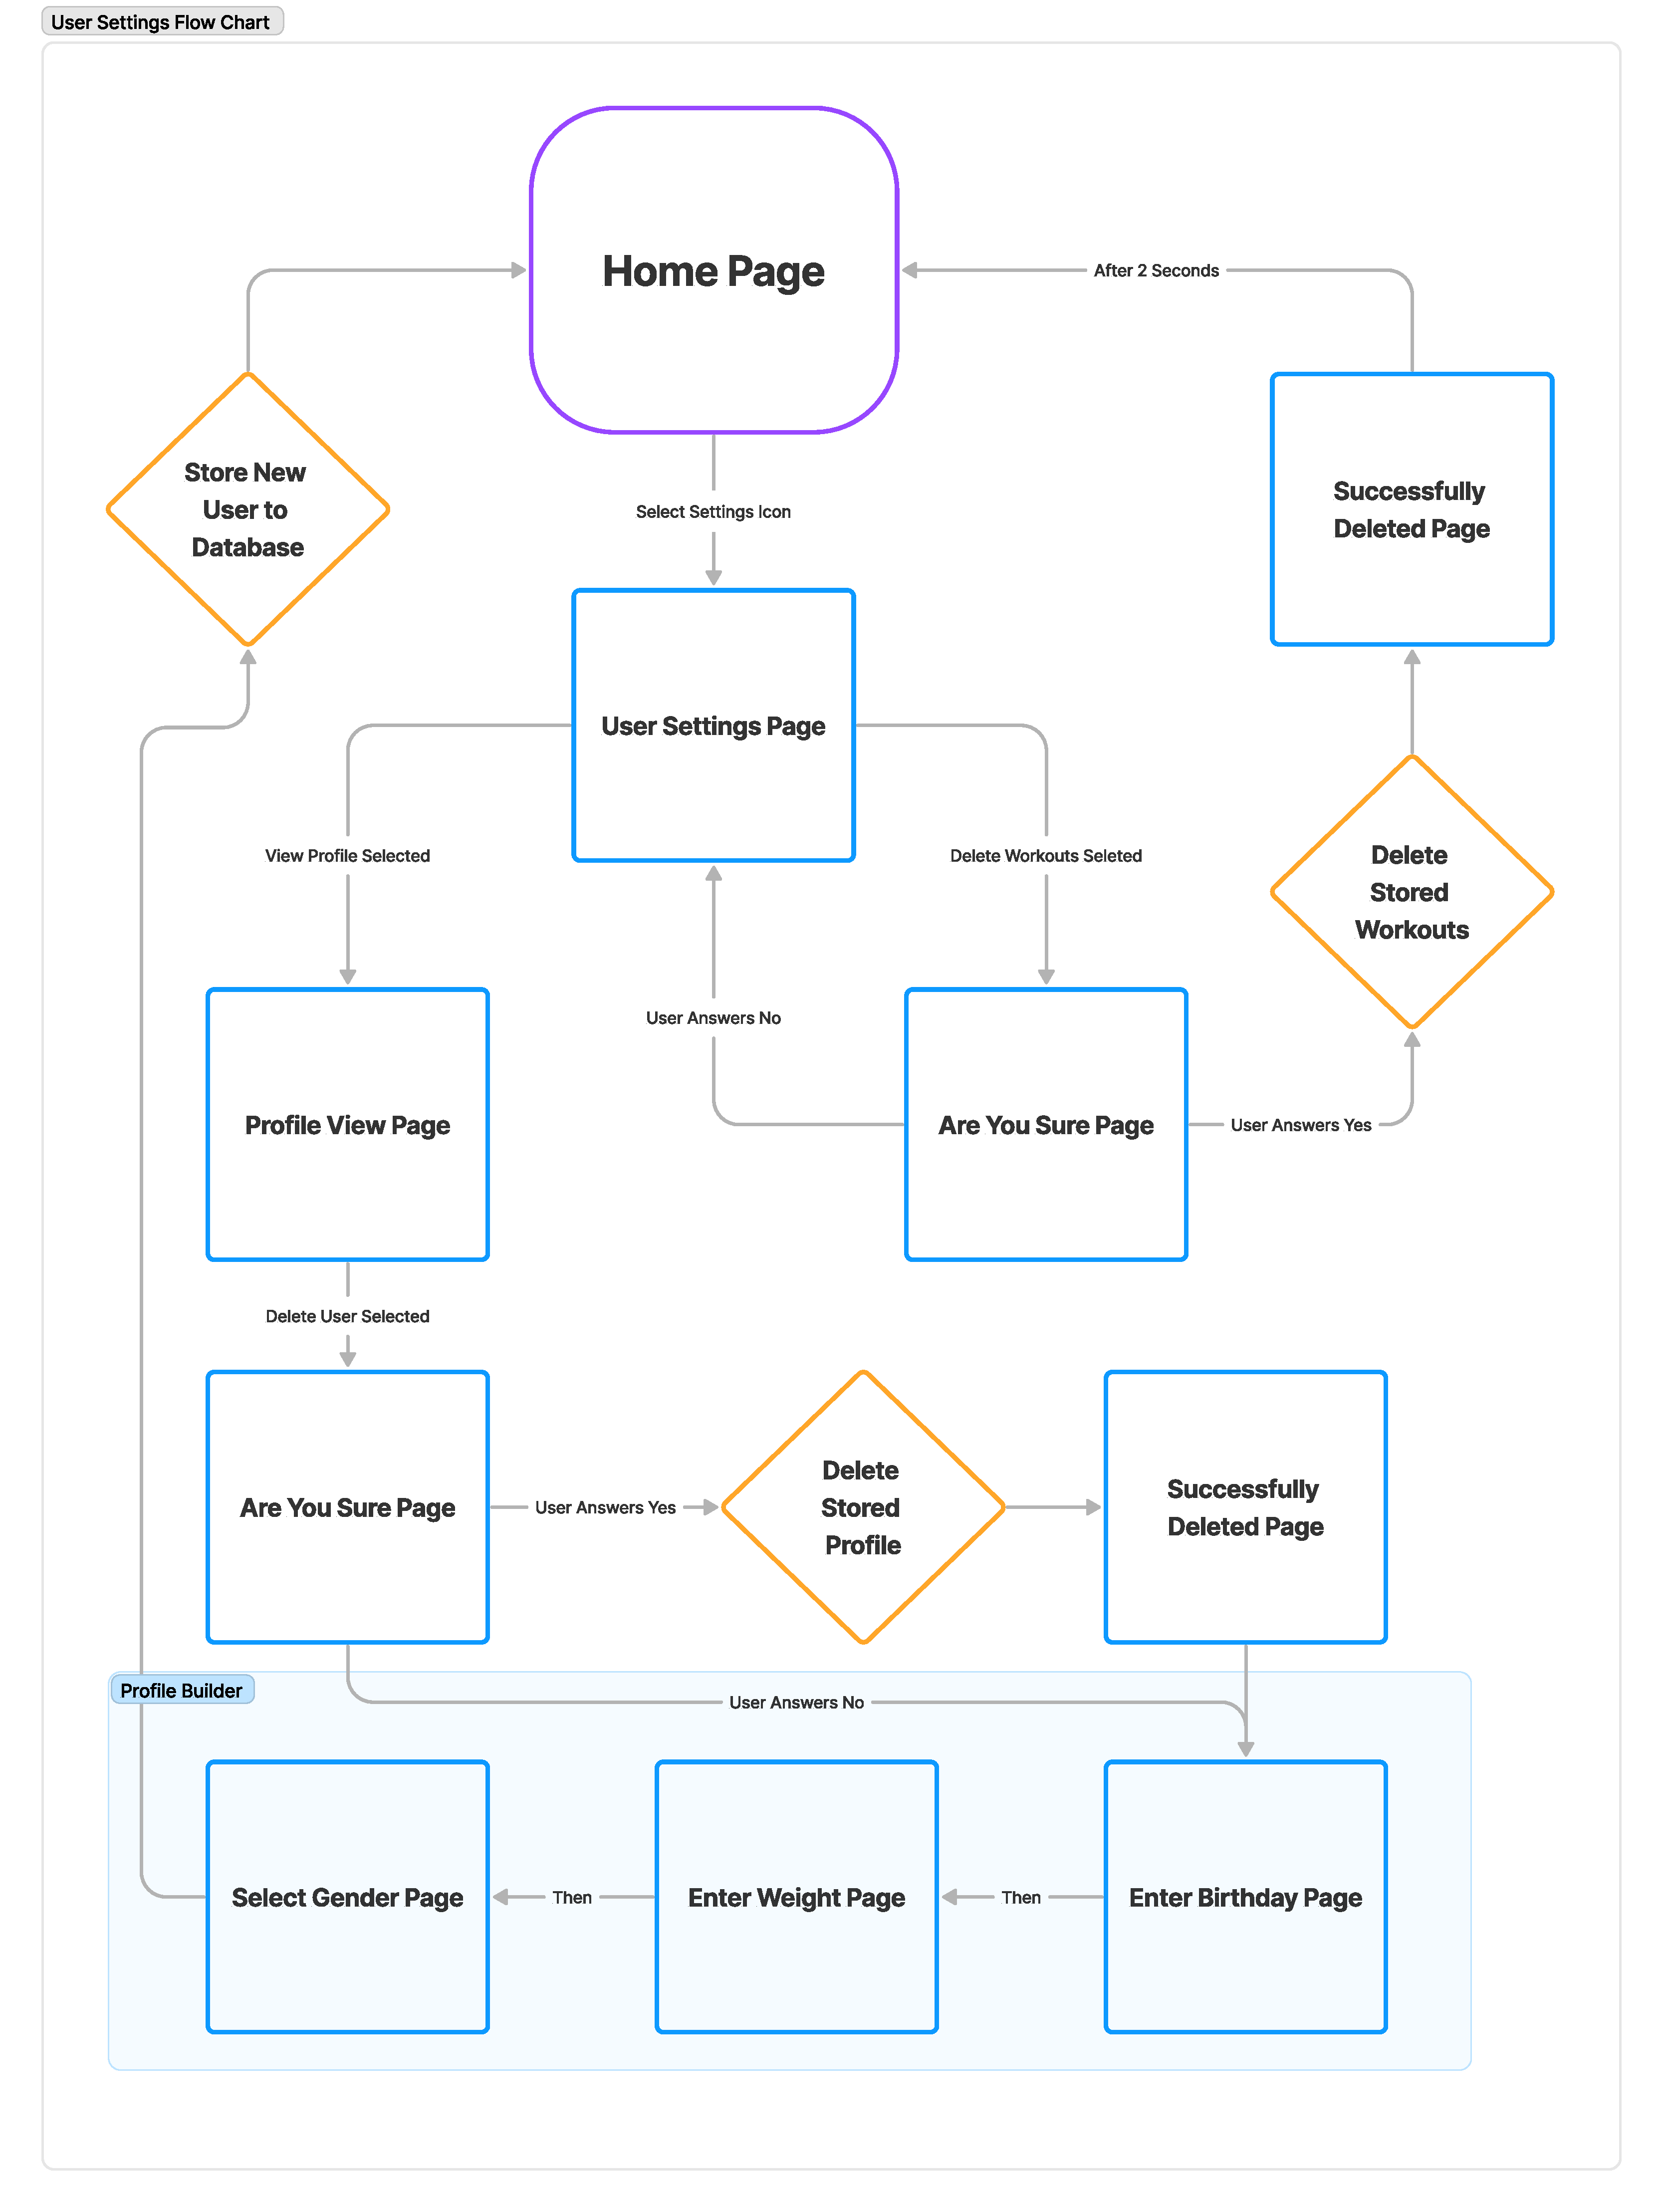
\includegraphics[width=0.75\linewidth]{dissertation//dissImages/UserSettingFlow.pdf}
    \caption{Enter Caption}
    \label{fig:enter-label}
\end{figure}

\end{appendices}

%==================================================================================================================================
%   BIBLIOGRAPHY   

% The bibliography style is abbrvnat
% The bibliography always appears last, after the appendices.

\bibliographystyle{abbrvnat}

\renewcommand{\thechapter}{0}
\bibliography{l4proj}

\end{document}
